\documentclass{article}
\usepackage[utf8]{inputenc}
\usepackage[margin=1in]{geometry}
\usepackage{siunitx}
\usepackage[autocite=superscript,backend=biber,sorting=none]{biblatex} % if lag: change biber to bibtex, recompile, the change back to biber and should be good!

\usepackage{hyperref}
\usepackage[noabbrev]{cleveref}
\usepackage{graphicx}
\usepackage{float}
\usepackage{pdflscape}
\usepackage{pdfpages}
\usepackage{titlepic}

\usepackage{fancyhdr, graphicx}
\renewcommand{\headrulewidth}{0pt}
\fancyhead[L]{}
\fancyhead[R]{

\includegraphics[scale=1.2]{Syntronic}
}
\pagestyle{fancy}

\title{%
	Braphy \\
	\large The python version of Braph 2.0}
\author{Alice Neimantaite \\ Lisa Sjöblom \\ Daniel Westerlund\\Syntronic R$\&$D, Gothenburg office}
\date{June 2020}
\titlepic{
\begin{figure}[h]
    \centering
    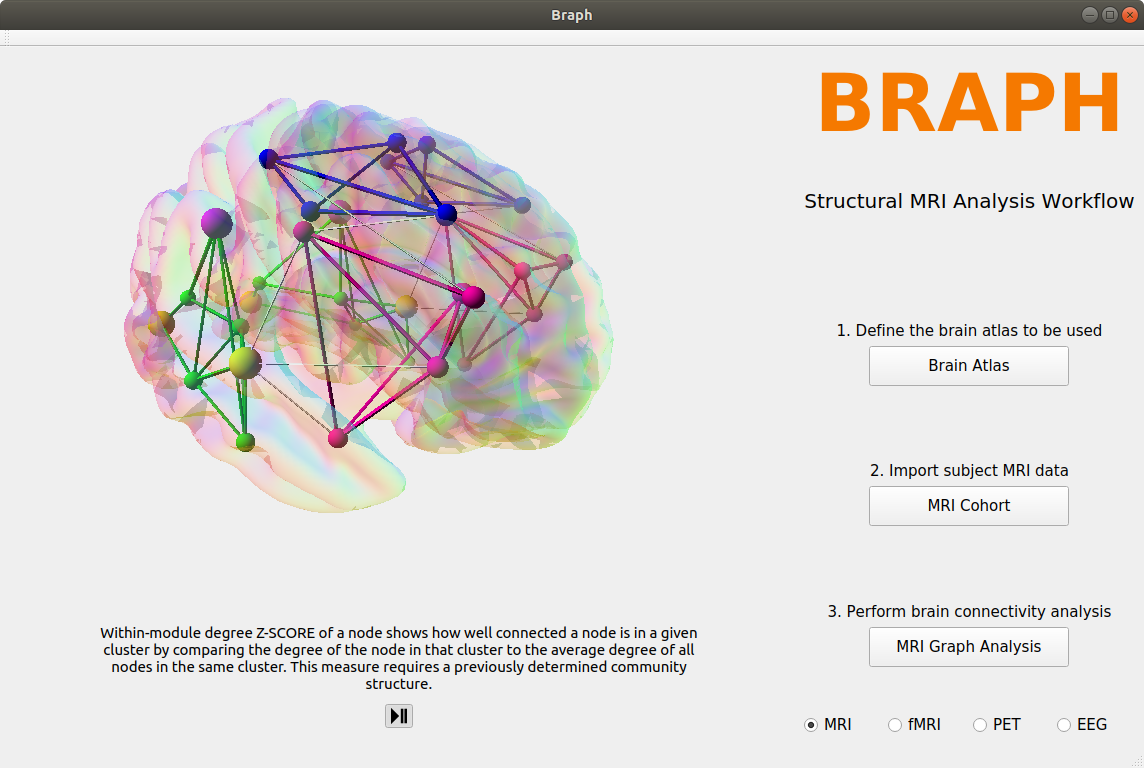
\includegraphics[width=\linewidth]{front_page.png}
    \caption{Start menu of Braphy}
    \label{fig:front_page}
\end{figure}
}


\begin{document}

\maketitle
\thispagestyle{fancy}
\clearpage

\section{Introduction}

For instructions on how to install and run the software, see the file 'README.md'.

This document describes the current state of the python version of Braph 2.0, or as we call it, Braphy. We focus on describing the parts that differ from Braph 1.0, and will therefore assume that the reader has previous knowledge about this software. The descriptions are relatively brief, and it could be a good idea to try the software out yourselves as you read it. We will mainly describe the software from the perspective of a person using the GUI, and not how it was implemented. In the future, our idea is that this document can be developed into a full manual of Braphy.

We have tried to finish the implementation for MRI and fMRI first, and have left the other data formats for the future. Hence, these are the only ones described here.

\section{Start Menu}

Figure \ref{fig:front_page} displays the start menu of Braphy. To the left, a rotating brain can be seen. The nodes, edges and text in the figure alters between a couple of different measures. If the pause button is pressed, the brain stops rotating. Once paused, the brain can be displaced using the mouse. Left click and drag to rotate it, scroll to zoom in or out, press mouse wheel and drag to pan in the x/y plane and ctrl + press mouse wheel and drag to pan in the x/z plane. These controls may be used anytime the brain view appears in the software.

To the right, the same buttons as in Braph 1.0 can be found. Note that so far, only MRI and fMRI are implemented. 

\section{Brain Atlas}

The brain atlas module in Braphy is very similar to the one in Braph 1.0, with a few differencies. The GUI can be seen in \cref{fig:brain_atlas}.

\begin{figure}[H]
    \centering
    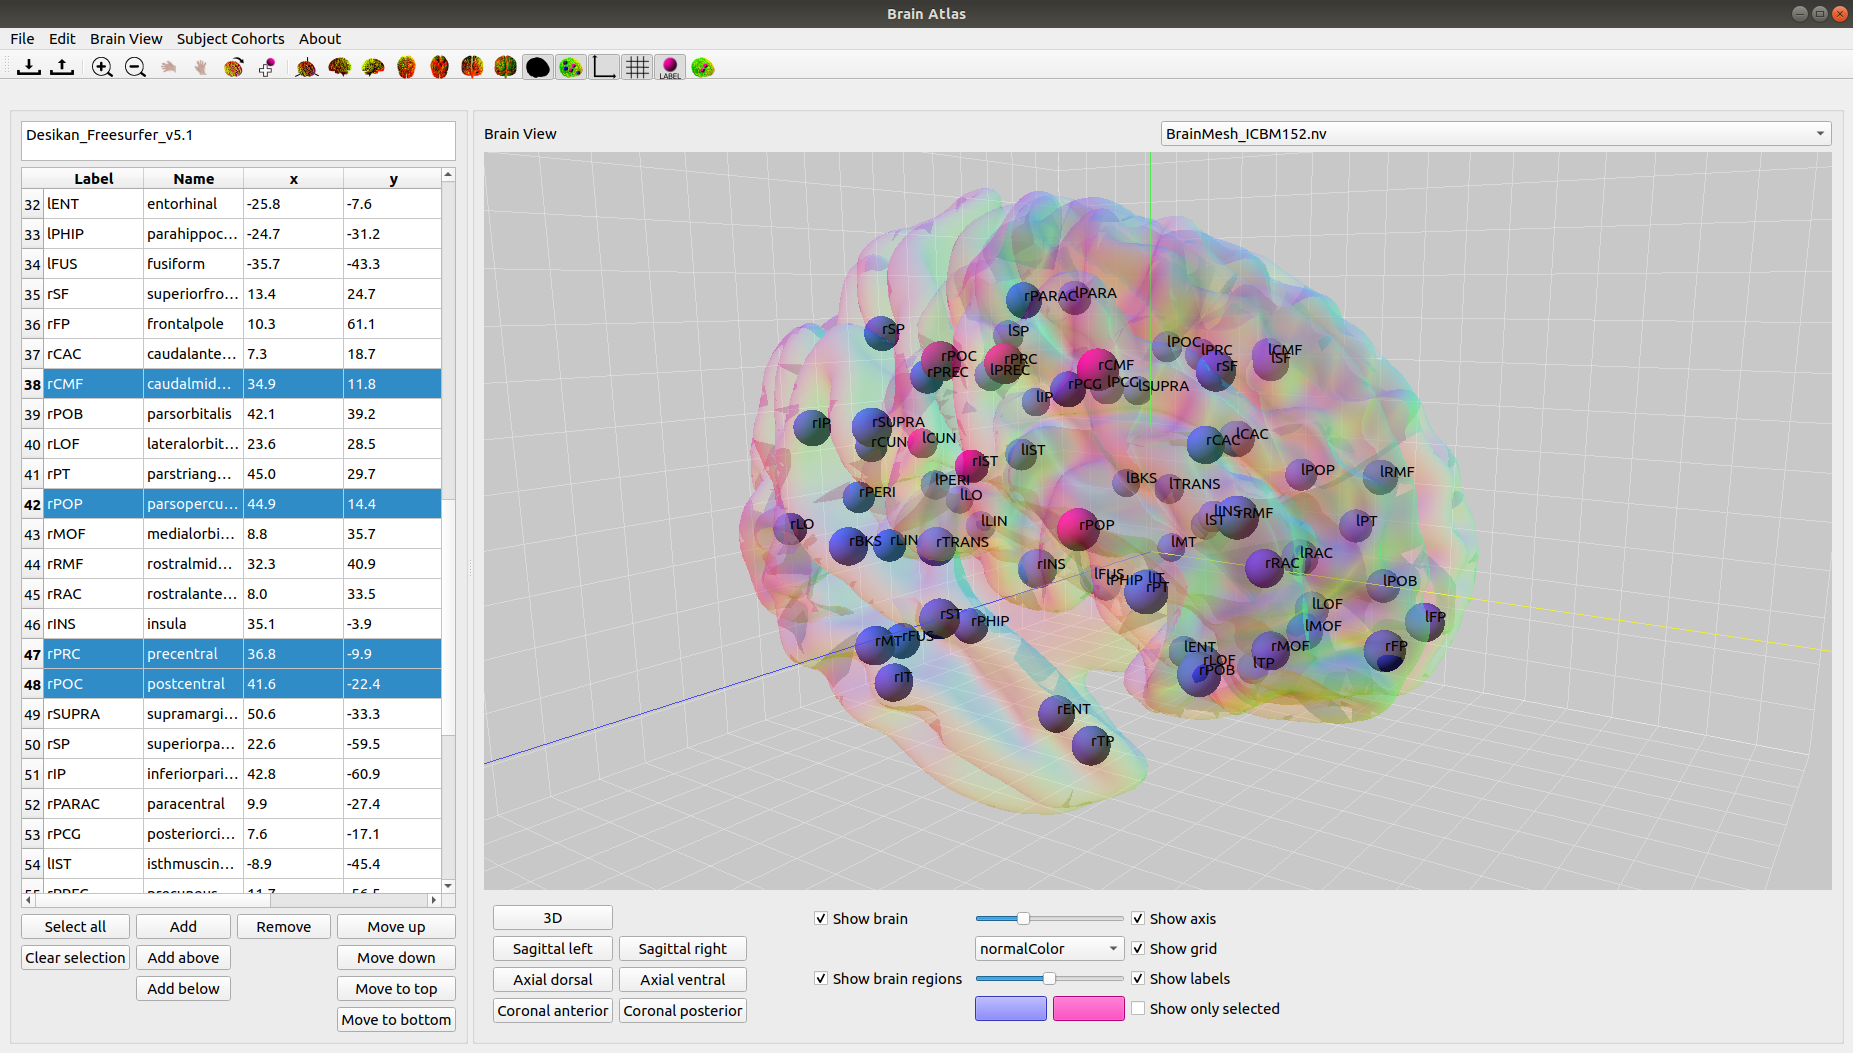
\includegraphics[width=0.9\linewidth]{brain_atlas.png}
    \caption{The Brain Atlas window. Six brain regions are selected. These are the pink ones in the brain view. They are also selected in the table to the left.}
    \label{fig:brain_atlas}
\end{figure}

First, we have created new icons for the buttons in the toolbar, located at the top of the window. These will be used throughout the software. They are available at Github and you are free to use them as well if you like. The toolbar has the same functionality as in Braph 1.0, but the one to the right is new. If you press it, only the selected brain regions will be visible in the brain view.

At the top right of the brain view, you can select a brain mesh. You can choose from meshes available in the software or load your own brain mesh.

The tools below the brain view is similar to the ones in Braph 1.0, and this panel will be used to control the brain view throughout the software. You can change the color of the brain mesh and the default and selected brain region colors.

There are no check boxes in the brain region table. Instead, select a region by simply clicking on it. To select several regions, press ctrl and click. This way of selecting rows in tables will be used several times in the software.

\section{MRI}

\subsection{MRI Cohort}

The MRI Cohort GUI can be seen in \cref{fig:mri_cohort_subject}, \cref{fig:mri_cohort_group} and \cref{fig:cohort_brain_view_down}. After selecting an atlas, the rest of the GUI becomes enabled. As long as no groups or subjects are added to the cohort, the user can change the atlas by pressing 'Select Atlas' again. Files in .atlas format are available in the repository.

There is only one button for loading subjects from file. By pressing it the user can load one or several files in the formats .txt, .xml or .xlsx.

The groups can be inverted, merged or intersected by using the buttons at the bottom left of the window. Select at least one group from the table above to enable the invert button, and at least two groups to enable the merge and intersect buttons. 

\begin{figure}[H]
    \centering
    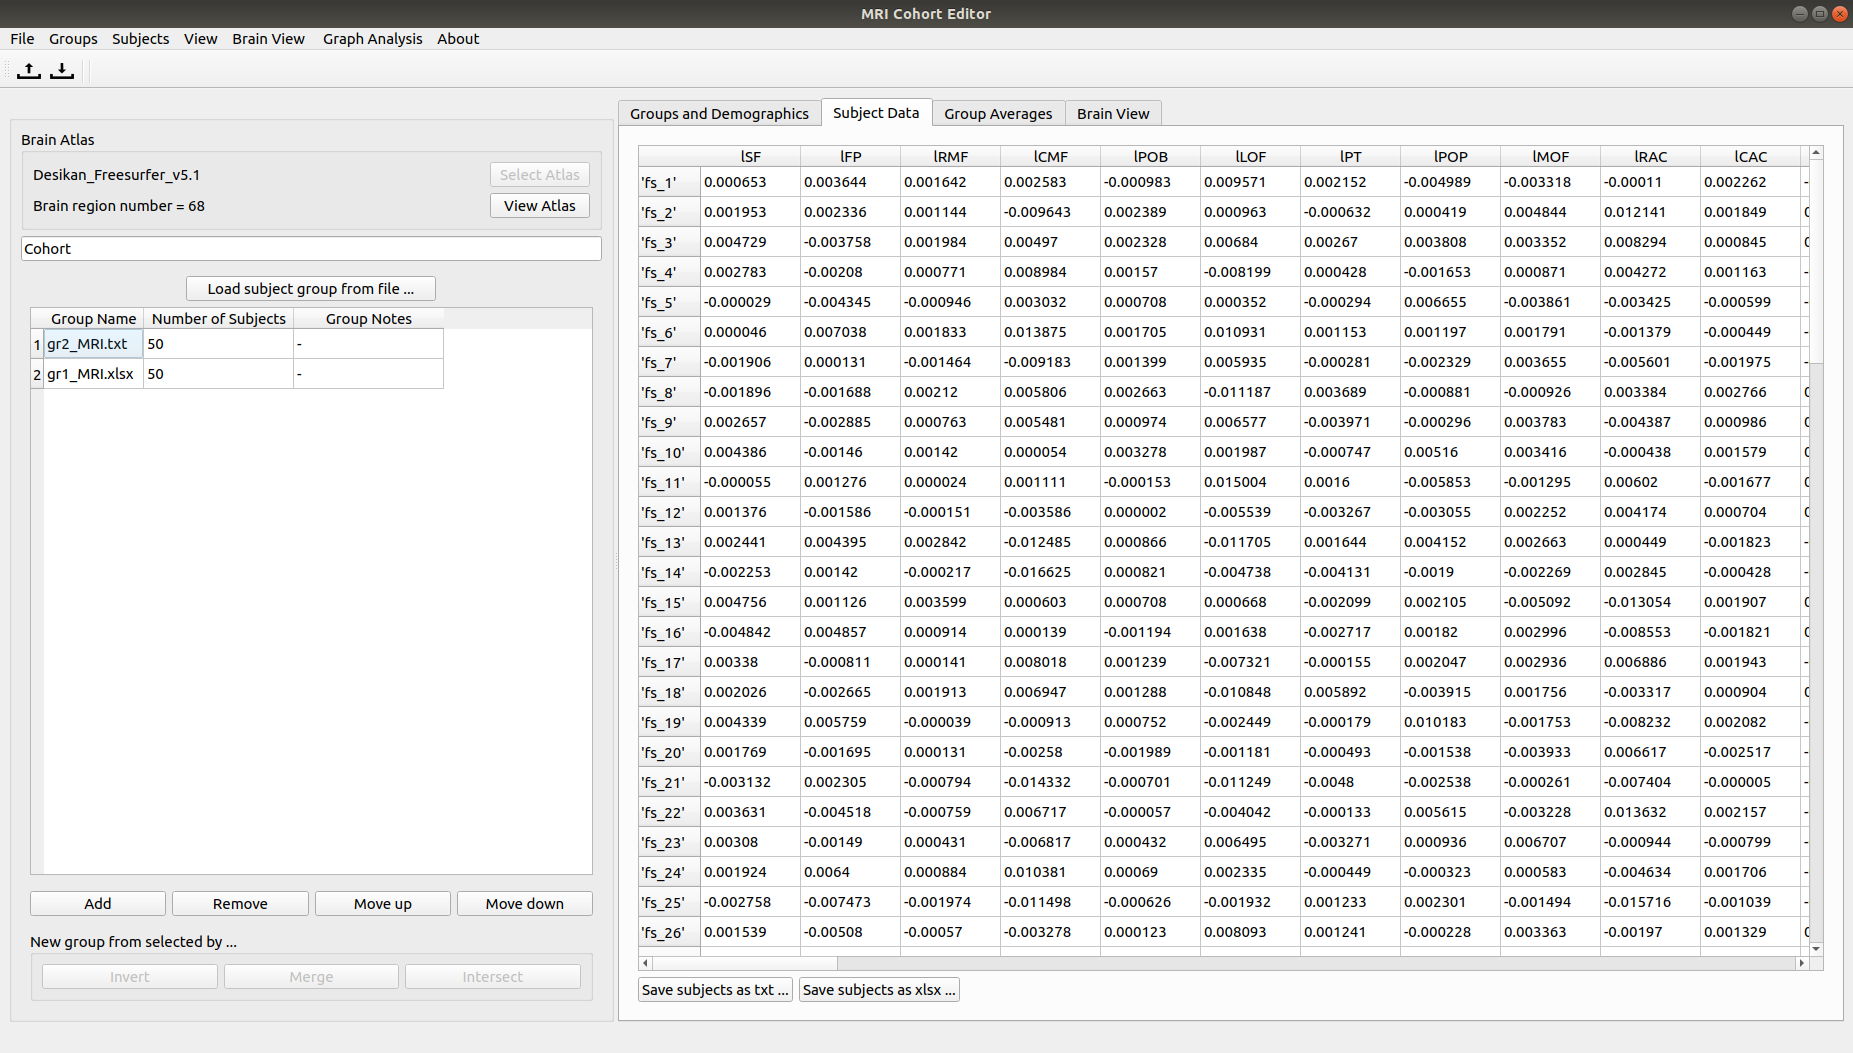
\includegraphics[width=0.9\linewidth]{mri_cohort_subject.png}
    \caption{The MRI Cohort Editor GUI. Here, the 'Subject Data' tab is selected. The subjects can be exported as .txt or .xlsx files.}
    \label{fig:mri_cohort_subject}
\end{figure}

\begin{figure}[H]
    \centering
    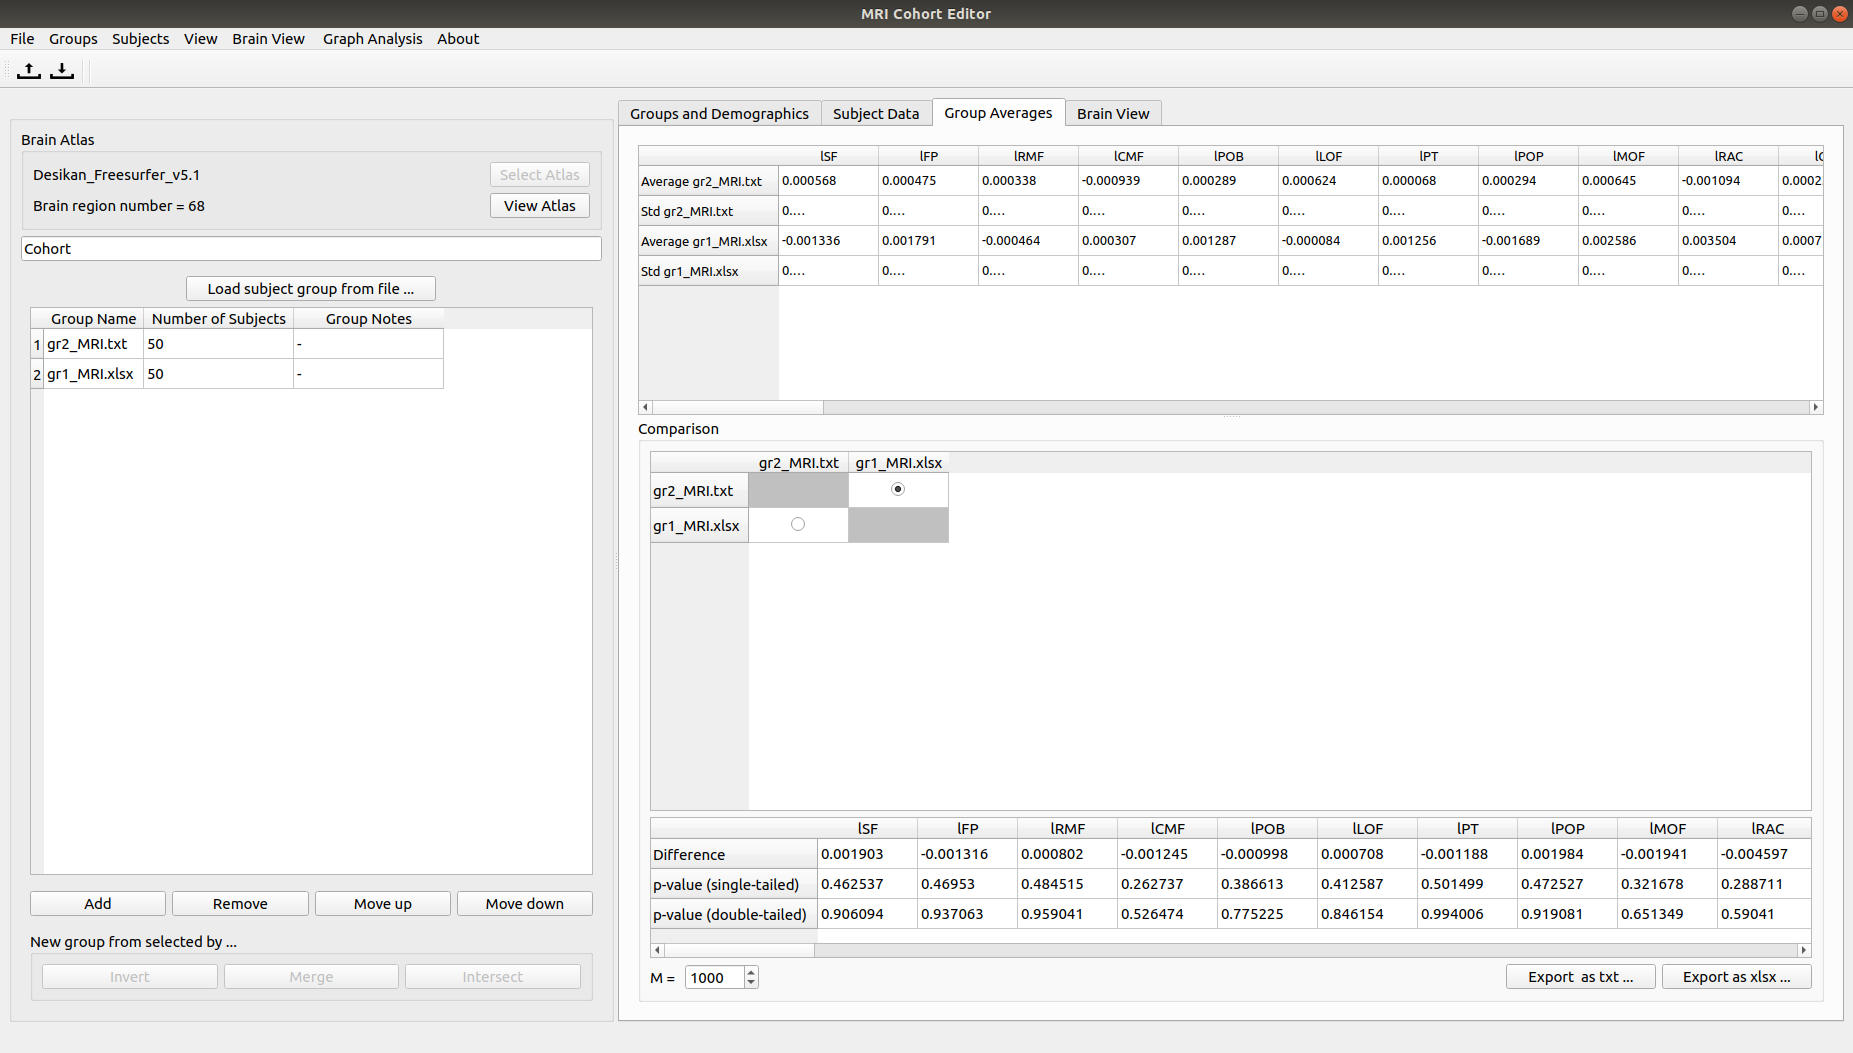
\includegraphics[width=0.9\linewidth]{mri_cohort_group.png}
    \caption{The MRI Cohort Editor GUI. Here, the 'Group Averages' tab is selected.}
    \label{fig:mri_cohort_group}
\end{figure}

\begin{figure}[H]
    \centering
    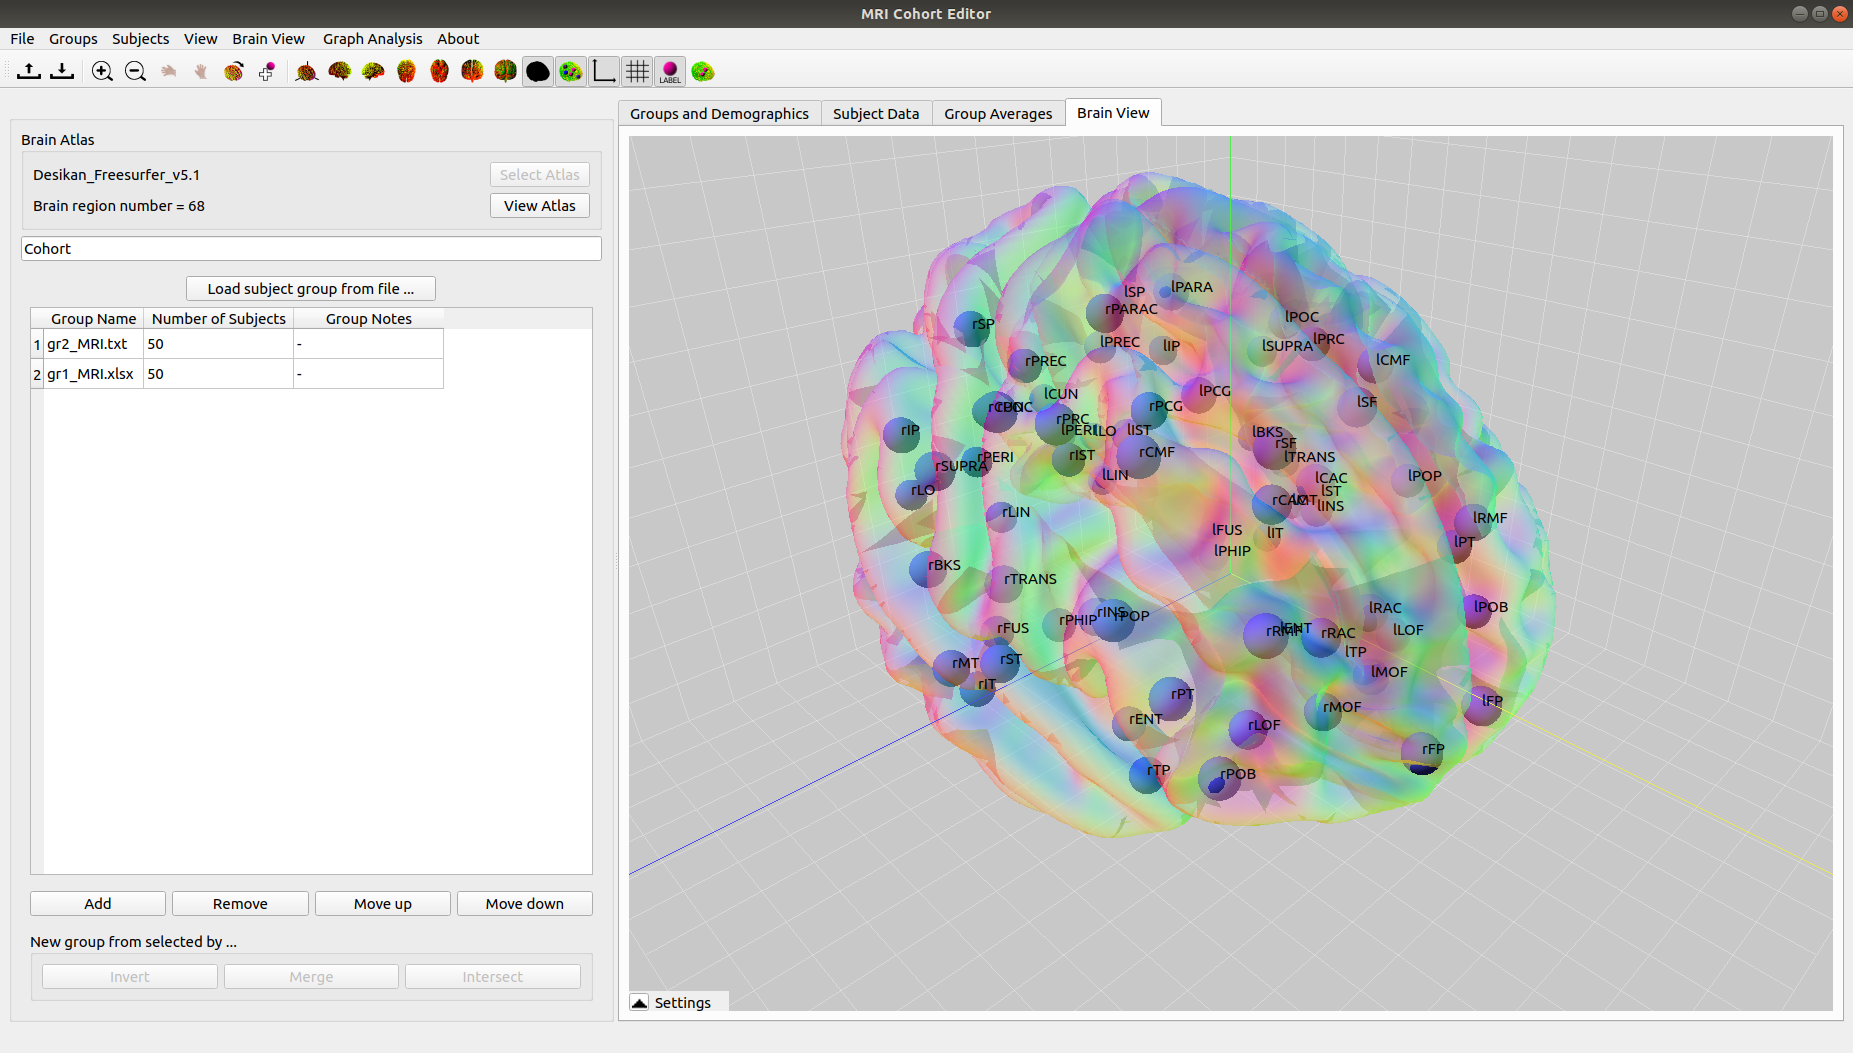
\includegraphics[width=0.9\linewidth]{cohort_brain_view_down.png}
    \caption{The MRI Cohort Editor GUI. Here, the 'Brain View' tab is selected.}
    \label{fig:cohort_brain_view_down}
\end{figure}

On the right side of the window, the different views are placed in separate tabs to make it clear what happens when you switch between them. In the tab 'Subject Data', see \cref{fig:mri_cohort_subject}, the subjects can be exported as .txt or .xlsx files.

The group averages tab has been split into three separate tables, see \cref{fig:mri_cohort_group}. The top one contains averages and standard deviations for all groups. In the second table, the user can select what groups to compare by pressing the radio buttons in the table. In the third table, the comparison of the two groups selected in the second table is displayed. By using the buttons on the bottom right of this tab the comparisons can be exported as .txt and .xlsx files. The files will contain the averages, standard deviations and comparisons of the selected groups.

The 'Brain View' tab is very similar to the brain view in the Brain Atlas GUI, see \cref{fig:cohort_brain_view_down}. Here, the settings are reached by pressing the small arrow next to the 'Settings' label. Once pressed, the plot settings appear. This window can be hidden by pressing the arrow again. The first tab of this window contains the same basic plot settings as the Brain Atlas GUI.

Here, the user can also select to visualize the subjects, groups or comparisons by size and/or color of the brain regions. In the second tab, see \cref{fig:cohort_vis_sub}, the subject data can be visualized by selecting a subject and visualization method (color or size). The colormap can be customed and the range of the brain region sizes can be set. In the 'Visualize groups' tab, see \cref{fig:cohort_vis_groups}, the average and/or standard deviation of a group can be visualized in a similar manner. In the last tab, the comparison of two groups can be visualized, that is the average, standard deviation, single p-value and double p-value. 

In these visualizations, the values are scaled such that the current largest node value always corresponds to the largest region size and/or color to the right of the colormap, and the smallest value to the smallest region size and/or color to the left of the colormap. Hence, it is not possible to compare different figures to each other.

\begin{figure}[H]
    \centering
    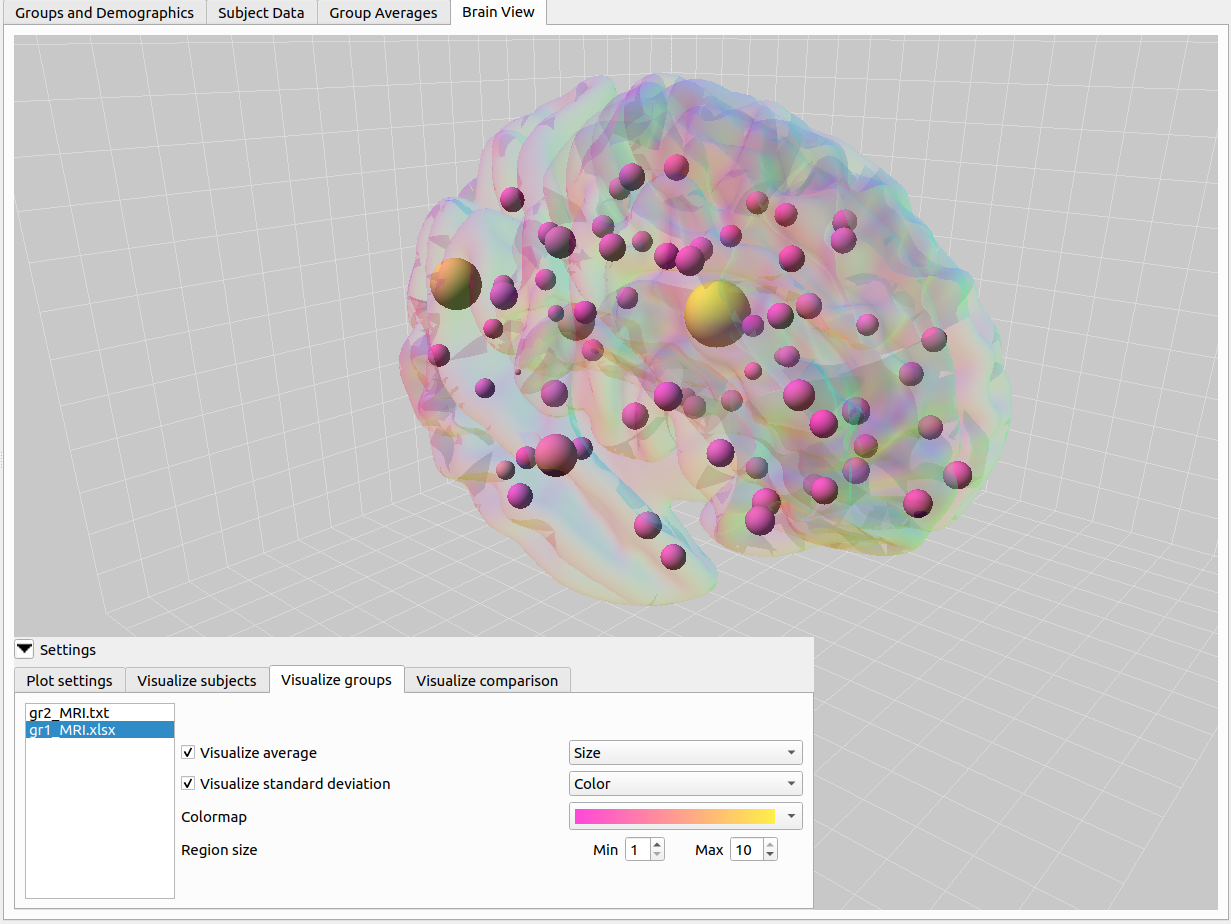
\includegraphics[width=0.9\linewidth]{cohort_vis_groups.png}
    \caption{The 'Brain View' tab with the settings window visible. Here, the averages and standard deviations of gr1\_MRI is visualized by different sizes and colors of the brain regions.}
    \label{fig:cohort_vis_groups}
\end{figure}

\begin{figure}[H]
    \centering
    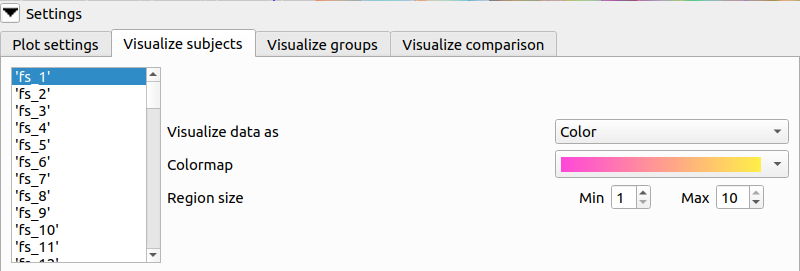
\includegraphics[width=0.7\linewidth]{cohort_vis_sub.png}
    \caption{Visualize subjects.}
    \label{fig:cohort_vis_sub}
\end{figure}

\begin{figure}[H]
    \centering
    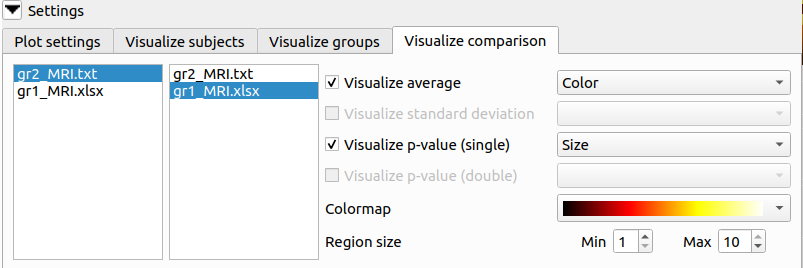
\includegraphics[width=0.7\linewidth]{cohort_vis_comp.png}
    \caption{Visualize comparisons.}
    \label{fig:cohort_vis_comp}
\end{figure}


\subsection{MRI Graph Analysis}
\label{sec:mri_ga}

When the MRI Graph Analysis GUI is opened, the only action available is to load a cohort or an analysis, see \cref{fig:locked}. Examples of cohort and analysis files for MRI are available in the repository. If you select and load a .cohort file, more options will be enabled, see \cref{fig:started}. If you select and load an .analysis file, you will skip ahead and go directly to \cref{sec:start_analysis} and \cref{fig:start_analysis}.

\begin{figure}[H]
    \centering
    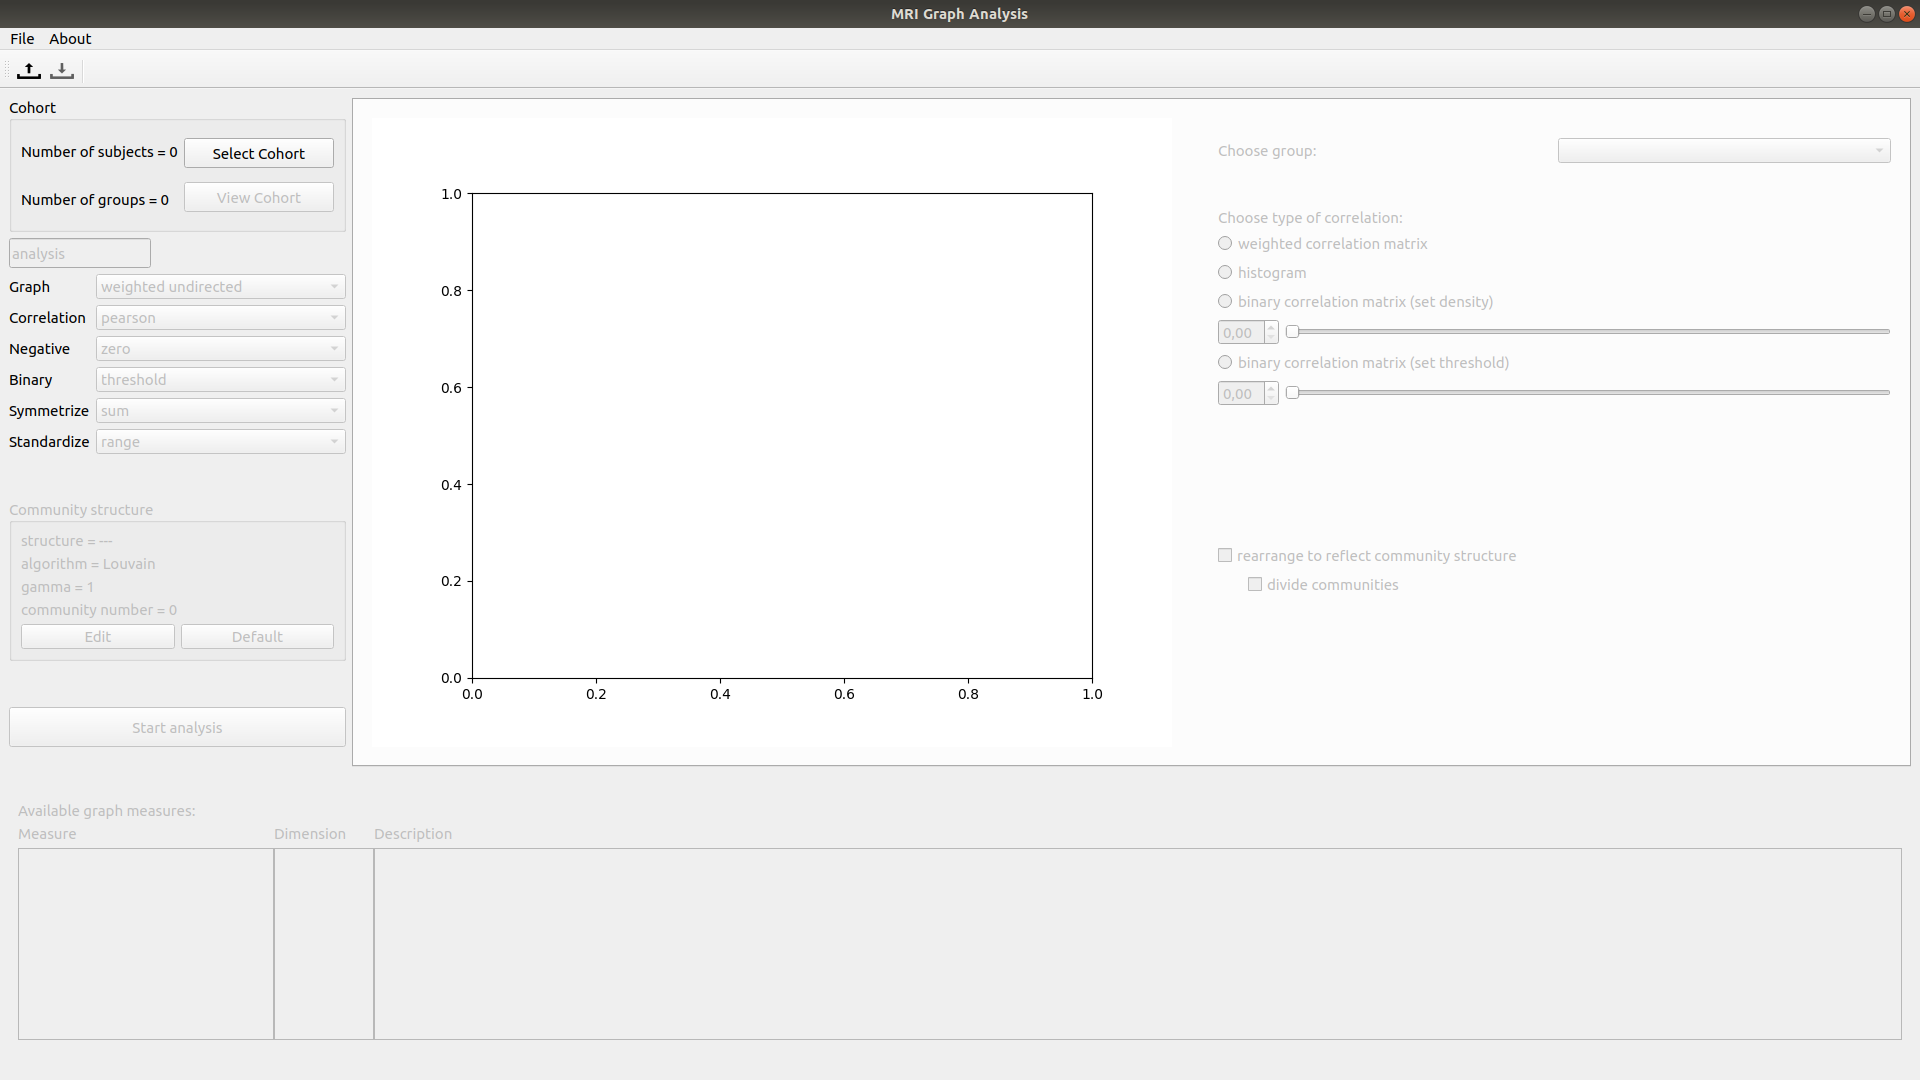
\includegraphics[width=0.9\linewidth]{graph_analysis_locked.png}
    \caption{The initial view in the graph analysis module.}
    \label{fig:locked}
\end{figure}

Let's assume that the user loads a .cohort file. The GUI is now in the state of \cref{fig:started}. In Braphy, we have added the 'View Cohort' button, so that you can select a new cohort if you change your mind. As you can see to the left in \cref{fig:started}, we have added the ability to change several graph settings. Only settings relevant for the current graph type are enabled. 

Further down, the 'Subgraph analysis' button has been removed. This button is instead added to the community structure window, which will be discussed later. 

At the bottom of the window, the measure table can be seen. Only the description of the selected measure is displayed, to avoid clutter.

The view of the correlation matrix and the corresponding settings to the right are only for visualization of the correlation. The settings here, such as the graph type and density, have no impact on the rest of the analysis. They only affect the plot of the matrix.

The toolbar is located at the top of the window. The first two icons correspond to opening and saving the analysis. Next, there is a set of buttons that lets the user alter the correlation matrix plot.

\begin{figure}[H]
    \centering
    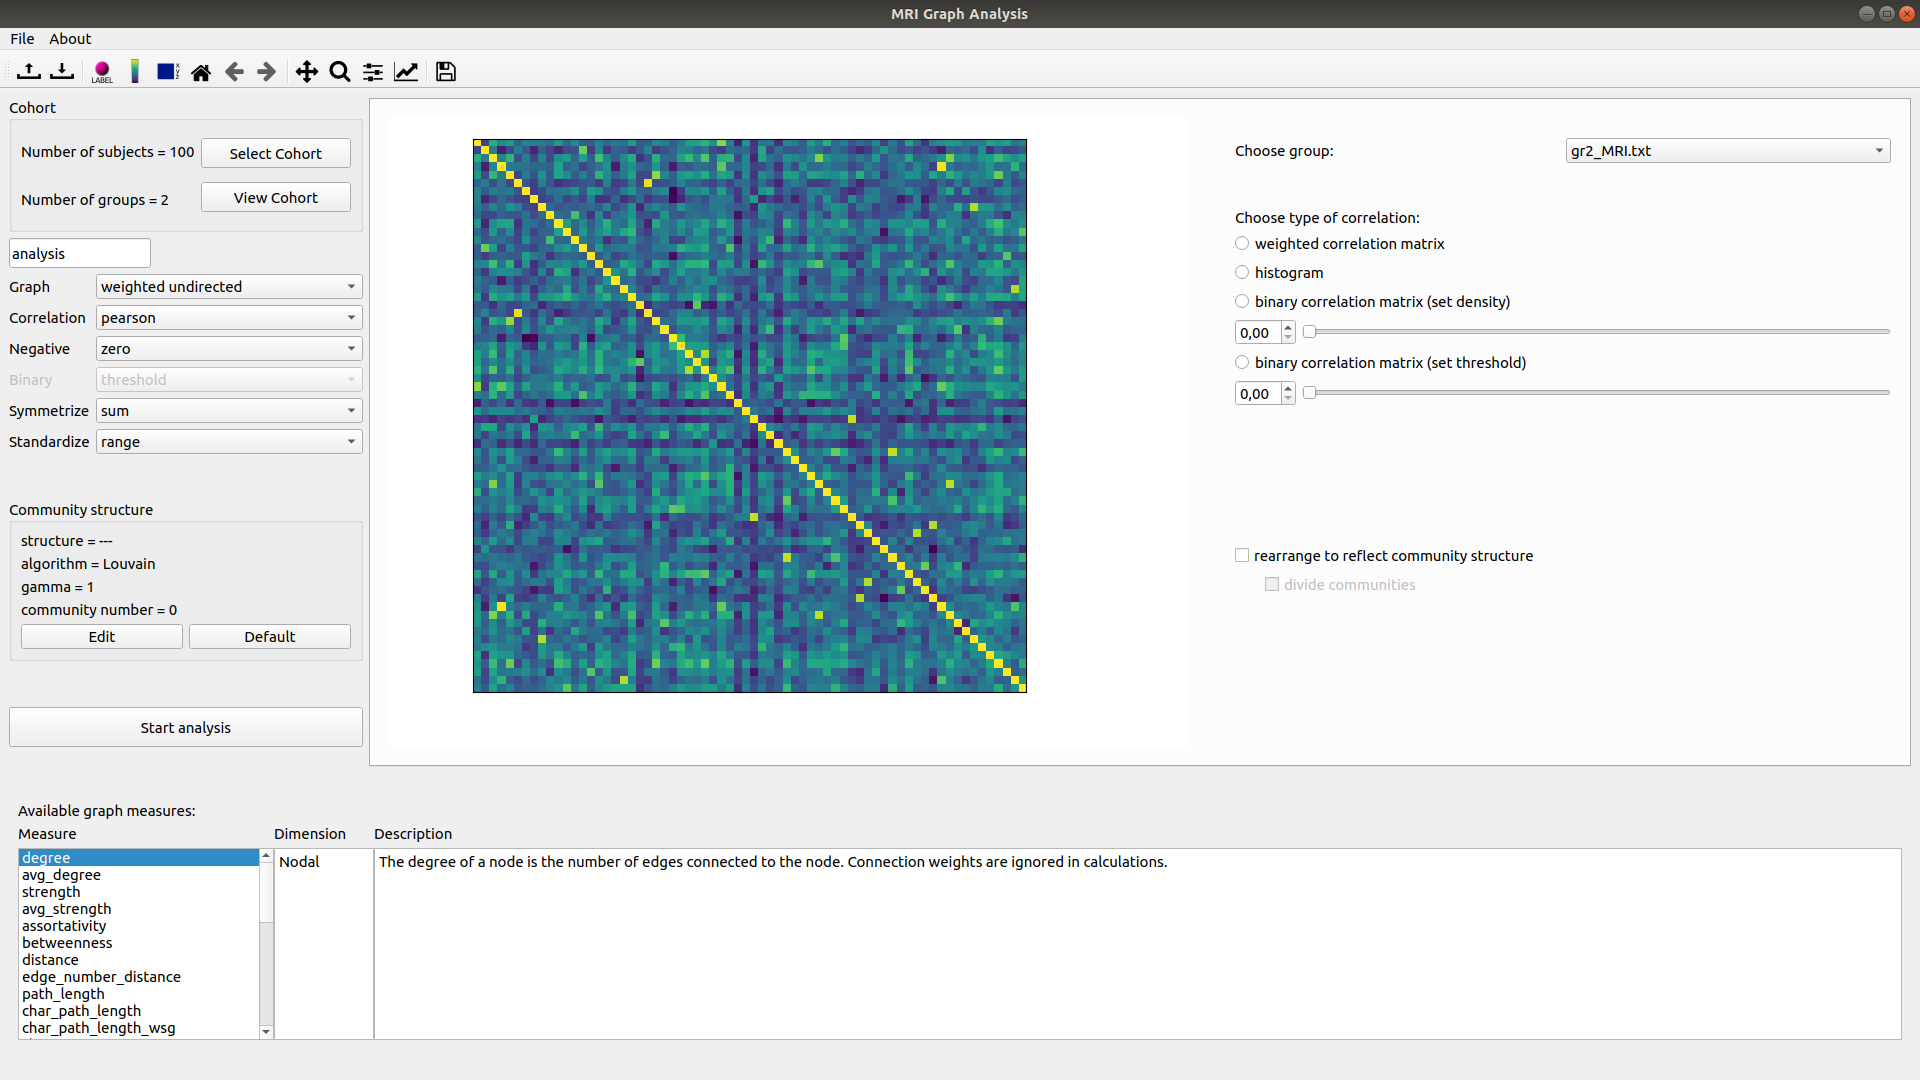
\includegraphics[width=0.9\linewidth]{graph_analysis_cohort.png}
    \caption{The graph analysis GUI after a cohort has been loaded.}
    \label{fig:started}
\end{figure}

\subsubsection{Community Structure GUI}

The community structure GUI is opened by pressing the 'Edit' button in the Graph Analysis GUI. It can bee seen in \cref{fig:community}. At the top of the window, there is a toolbar which contains buttons that lets the user alter the brain view. For example, you can change the viewpoint, zoom in and out, choose wether to show the brain mesh or not and so on.

As before, options for the visualization is reached by pressing the arrow next to the 'Settings' label. In the 'Plot settings' tab, basic brain view settings can be found. In the 'Visualize communities' tab, see \cref{fig:vis_com}, colors for each community can be defined by pressing on the colored buttons. Note that this tab has to be selected to visualize the communities. 

To edit the communities, use the tools to the bottom left in \cref{fig:community}. Start by selecting what group you want to define the community structure for. Next, choose if you want to use a fixed or a dynamic structure. Here, the fixed structure corresponds to a structure that can be altered manually by the user. A dynamic structure means that the communities are computed according to the selected algorithm and gamma value. Currently, only the Louvain algorithm is implemented. Next, the user can save the community structure displayed in the table. You can either set this structure for the current group, by clicking the button 'Set for current', or you can set it for all groups by clicking the button 'Set for all'. If you click 'Reset', the table shows the latest saved community structure for the current group. Note that in order to visualize the communities in the brain view, you have to save them first.

Since this is implemented slightly different than in Braph 1.0, we would like your input on our approach. The reason we did it this way is that we wanted to give more flexibility to the user. For example, you can now use a manually defined community structure for one group and a dynamically computed structure for another group. On the downside, this means that we have to save a community structure for each group in memory. This will be a matrix of size nodes*groups (and nodes*subjects for fMRI).

In the future, it might also be desireable to have the option "compute and set all communities separately but with the same algorithm and gamma value", although this is not implemented yet.

The subgraph analysis can be opened from this window, by selecting a column that includes the nodes that you want to use in the subgraph and then pressing 'Start subgraph analysis for selected community'.

\begin{figure}[H]
    \centering
    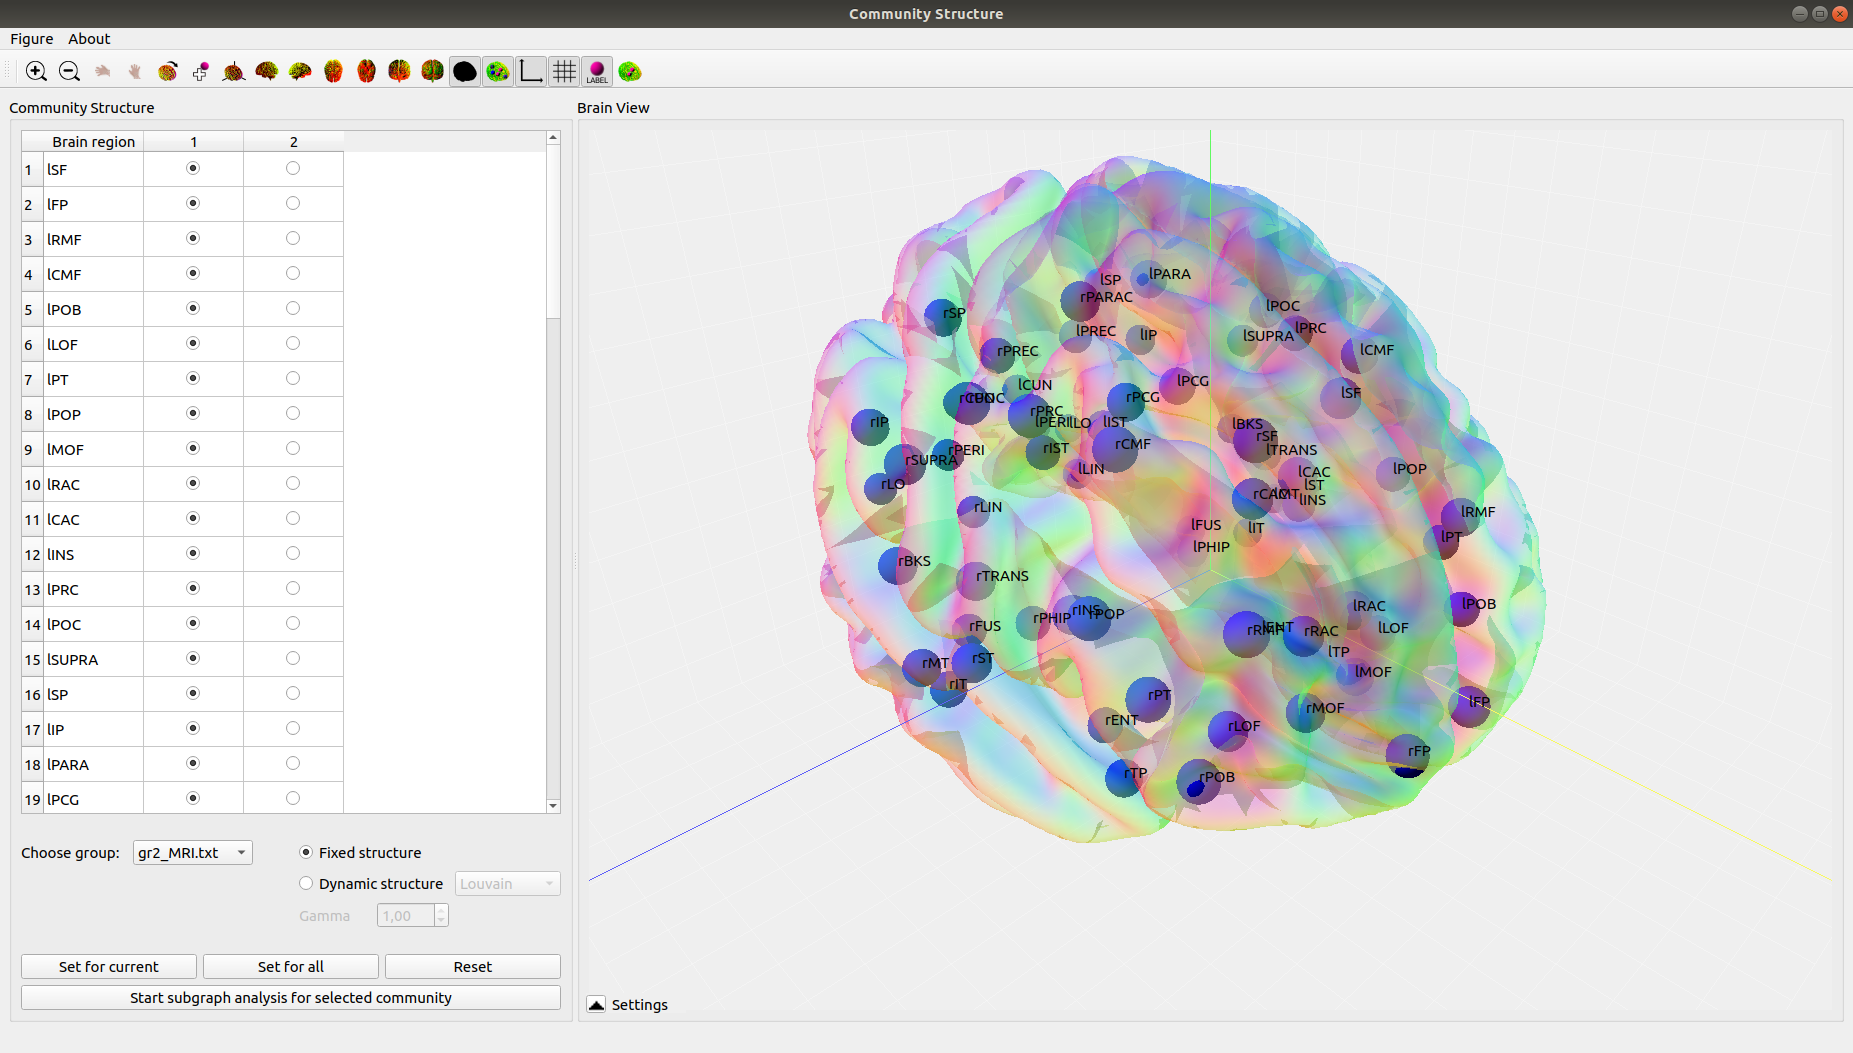
\includegraphics[width=0.9\linewidth]{community_structure.png}
    \caption{The community structure GUI.}
    \label{fig:community}
\end{figure}

\begin{figure}[H]
    \centering
    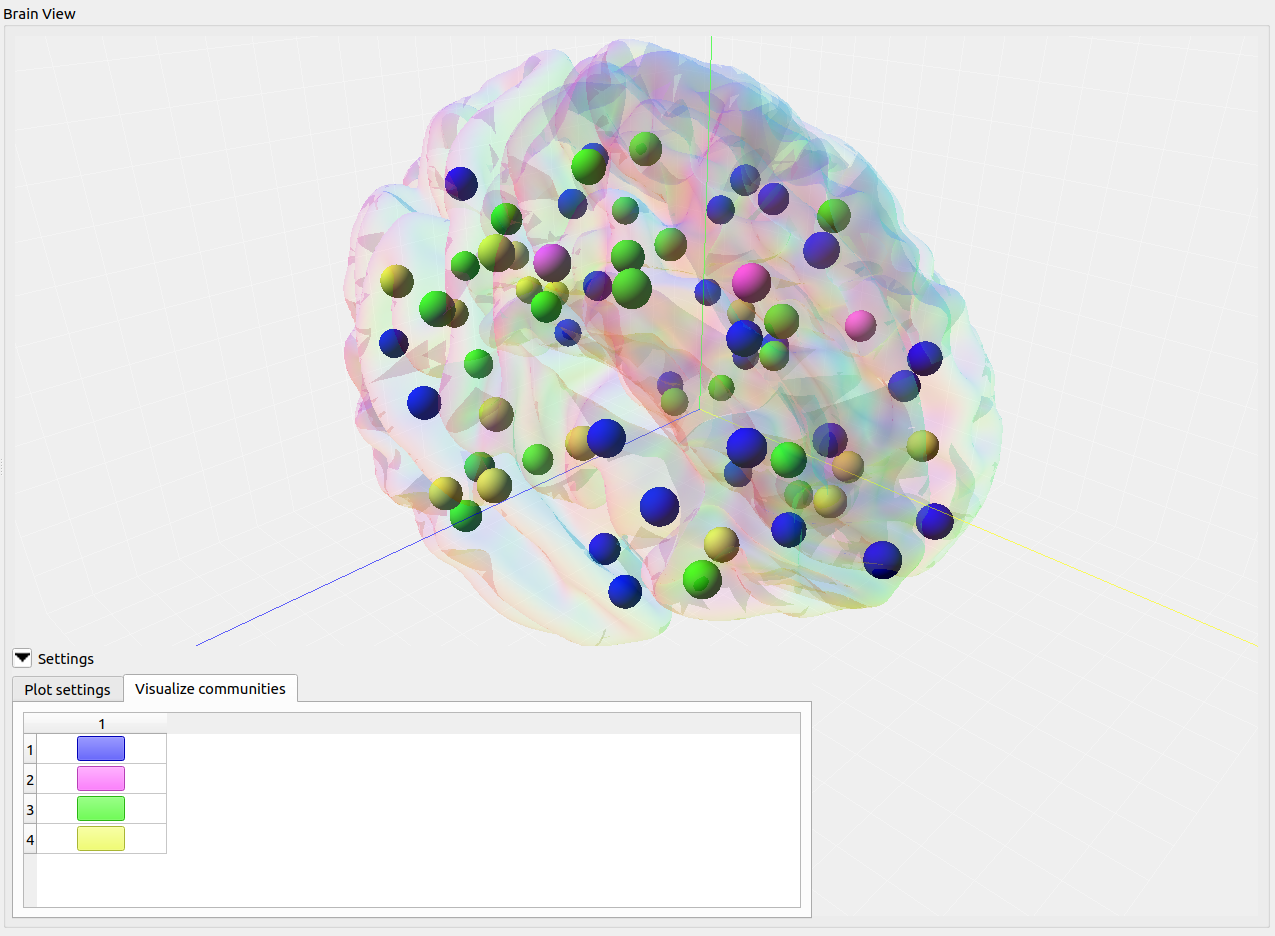
\includegraphics[width=0.8\linewidth]{visualize_communities.png}
    \caption{Using the visualize communities tab, the color of the nodes can be set corresponding to their communities.}
    \label{fig:vis_com}
\end{figure}

\subsubsection{Start Analysis}
\label{sec:start_analysis}

If you press the 'Start analysis' button in the Graph Analysis GUI, you lock the graph settings and community structure, see \cref{fig:start_analysis}. In Braph 1.0 this opened a new window, but we have chosen to alter the existing window instead, since they are so similar. 


The table of measures don't have a column of descriptions here. Instead, if you hold a cursor over the name of a measure, a description of it appears. 

The random comparison is not yet implemented. We are still working on the algorithm for randomization of graphs, and are also waiting to see how you will implement the random comparison (refering to email conversation a few weeks ago).

In the calculation windows, no progress report or timing has been added yet. They will only print 'DONE' once the calculations are finished. Also, the calculations can not be paused/resumed. 

In the tabs Global, Nodal and Binodal measures, measures and comparisons that are already computed can be seen. These tables and the settings in them are similar to Braph 1.0. The graphs for binary graphs has not been implemented yet. The binodal tab is added, and works in the same way as the nodal one, with an additional brain region selection. 

The 'Notes' column in the tables is not yet implemented, but the idea is that the user should be able to write and save notes in this column. The 'Param' column is not implemented yet either. We are not sure of what should be put here.

The data in these tables can be exported as .txt or as .xlsx files. The data in the exported files will be exactely the rows and columns that are displayed in the table. An idea that we have for the future is that you should be able to export all computed measures/comparisons at once here, and not only the ones that are currently displayed in the tables. Perhaps you know best what kind of export alternatives that could be useful here?

\begin{figure}[H]
    \centering
    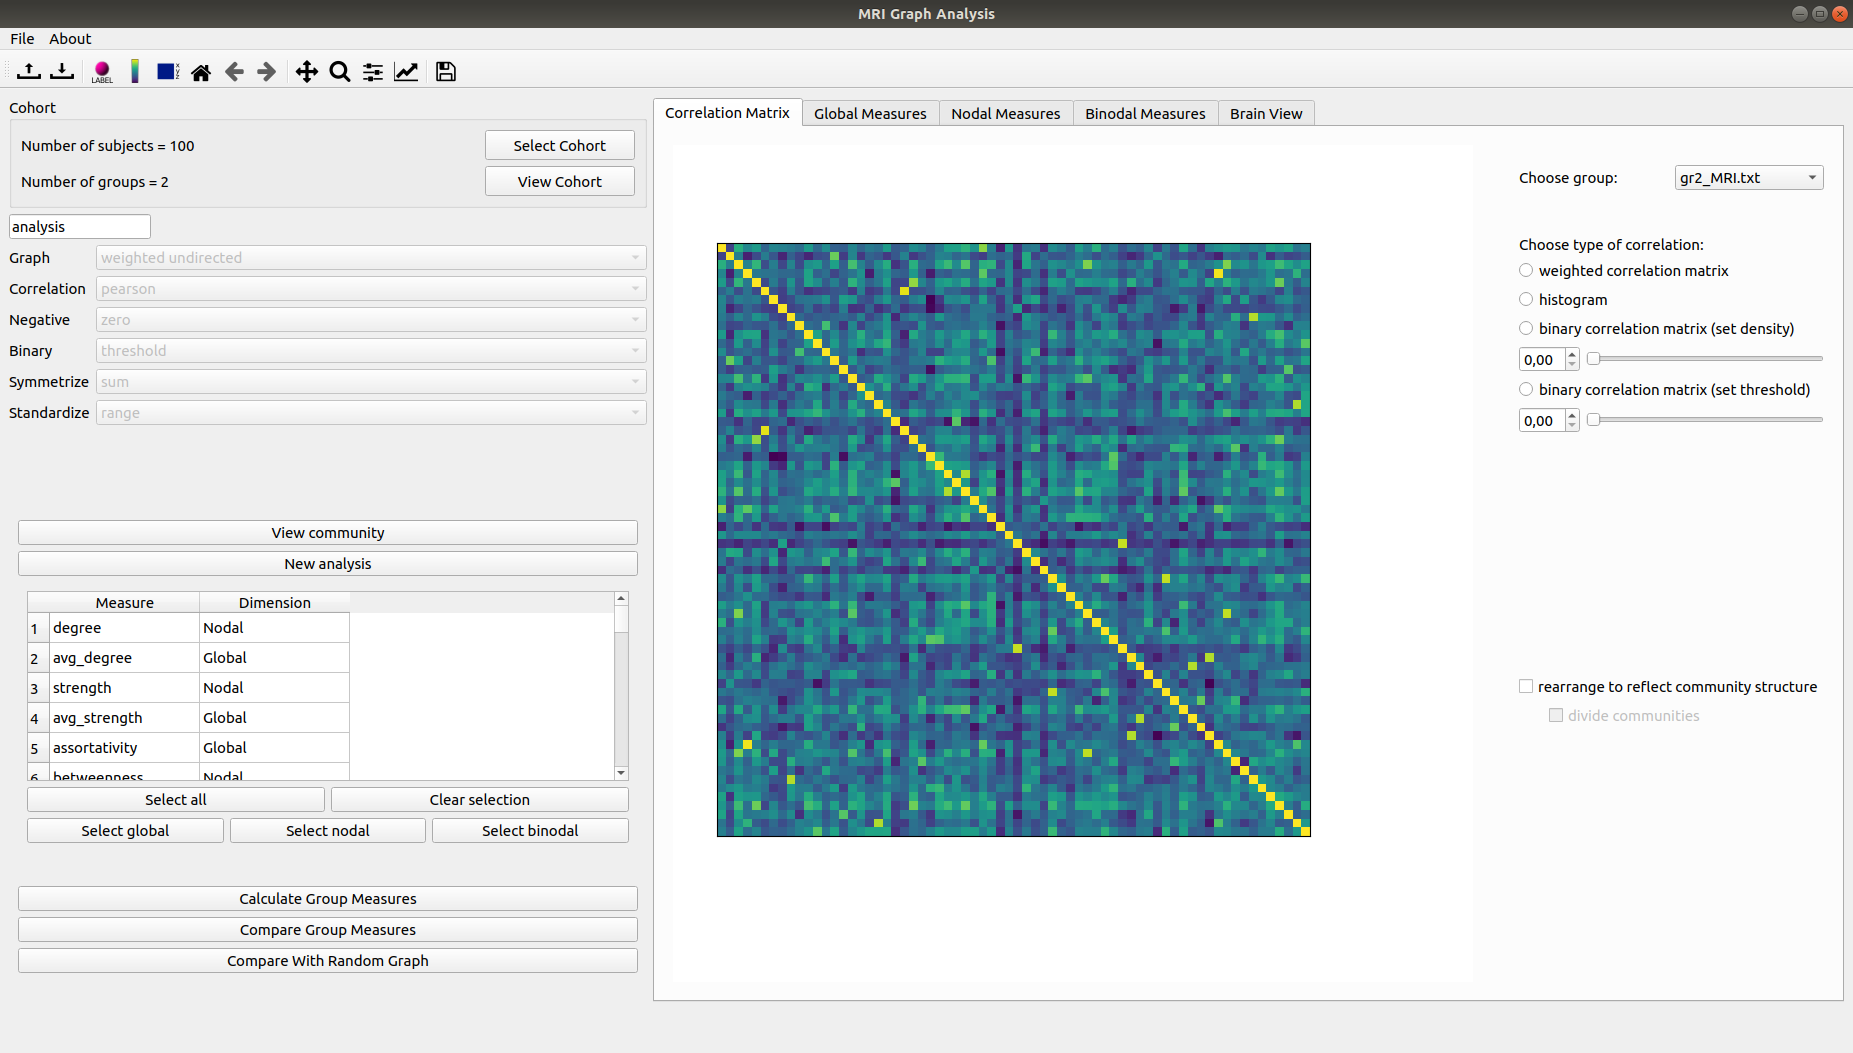
\includegraphics[width=0.9\linewidth]{start_analysis.png}
    \caption{The graph analysis GUI after the start analysis button has been pressed. The graph settings and the community structure is fixed, and additional tabs behind the correlation matrix can be selected. The corresponding view in Braph 1.0 was a new window.}
    \label{fig:start_analysis}
\end{figure}

In the last tab, different visulizations can be made. Like before, press the arrow to see the settings. The 'Plot settings' tab is identical to before. In the next tab, the graph can be visualized, see \cref{fig:graph_vis}. Hopefully, the settings here are self explanatory. Unfortunately, this is a bit slow for weighted graphs and graphs with high density.

\begin{figure}[H]
    \centering
    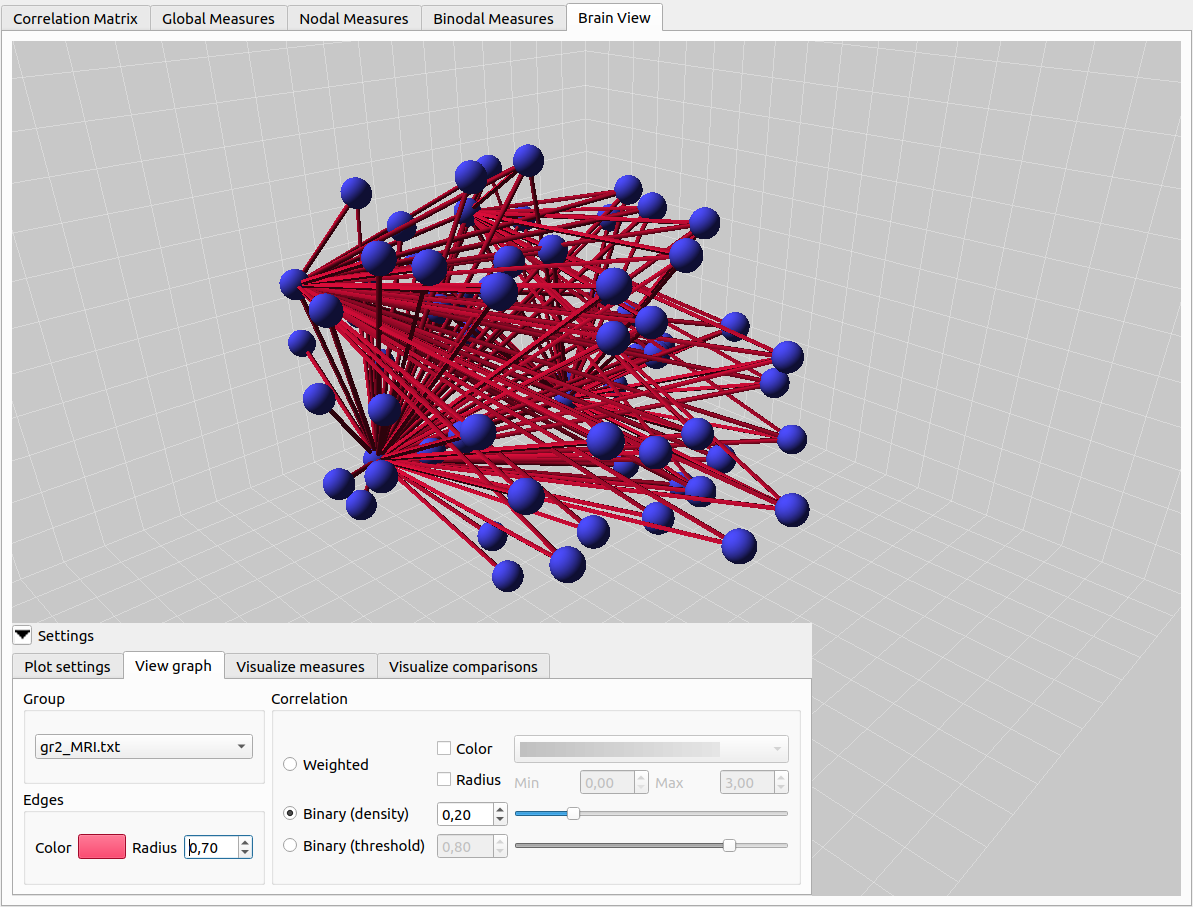
\includegraphics[width=0.65\linewidth]{graph_vis.png}
    \caption{3D visualization of the graph of the specified group. The brain mesh has been removed for a better view of the graph, but could be shown as a transparent surface above it. This is altered in the 'Plot settings' tab.}
    \label{fig:graph_vis}
\end{figure}

In the tabs 'Visualize measures' and 'Visualize comparisons', see \cref{fig:measure_vis} and \cref{fig:comparison_vis}, nodal measures and comparisons can be visualized. This works similarly to the visualization in the cohort. Only measures and comparisons that are already computed can be selected here. The user can select to visualize the values by size and/or colors of the brain regions. For the comparisons, the difference between the groups and single and double tailed p-values can be visualized.

\begin{figure}[H]
    \centering
    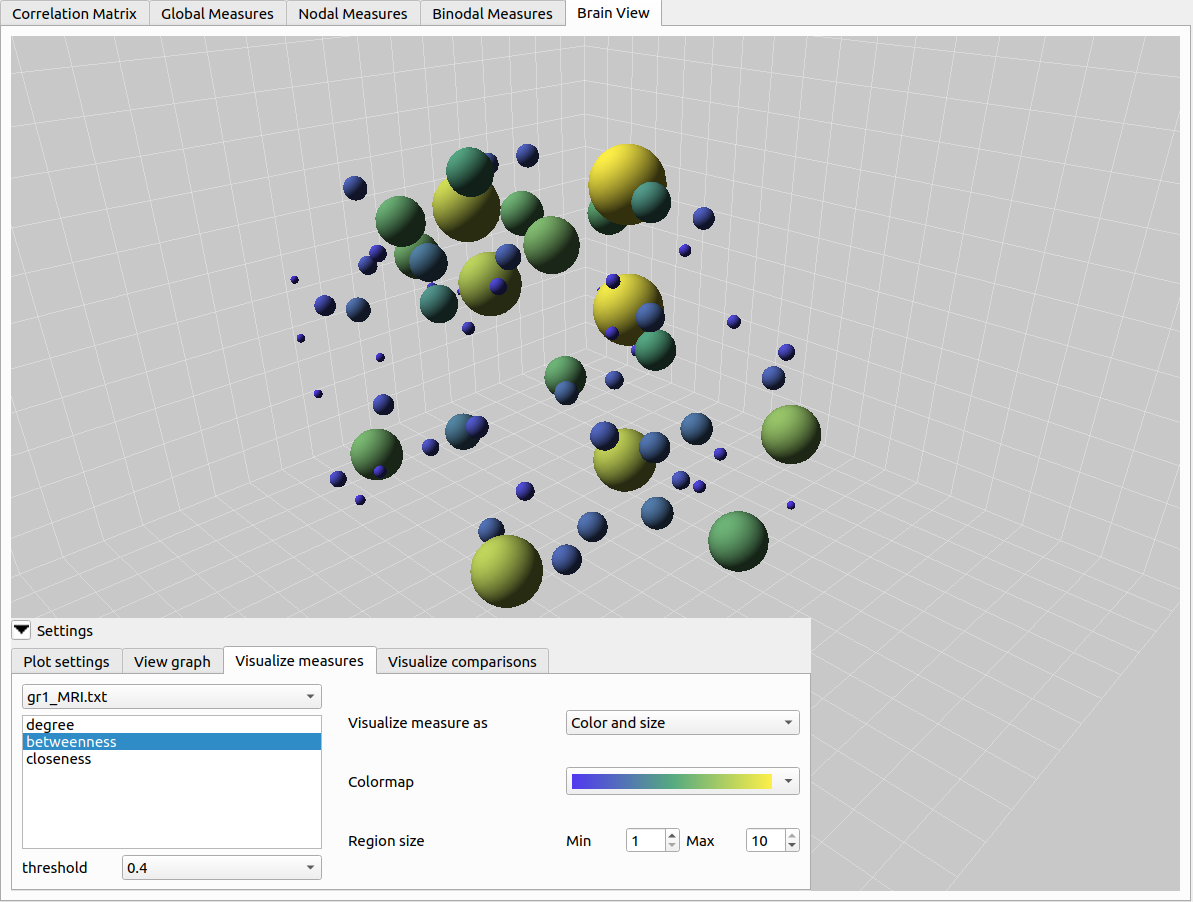
\includegraphics[width=0.7\linewidth]{measure_vis.png}
    \caption{Visualization of nodal measures.}
    \label{fig:measure_vis}
\end{figure}

\begin{figure}[H]
    \centering
    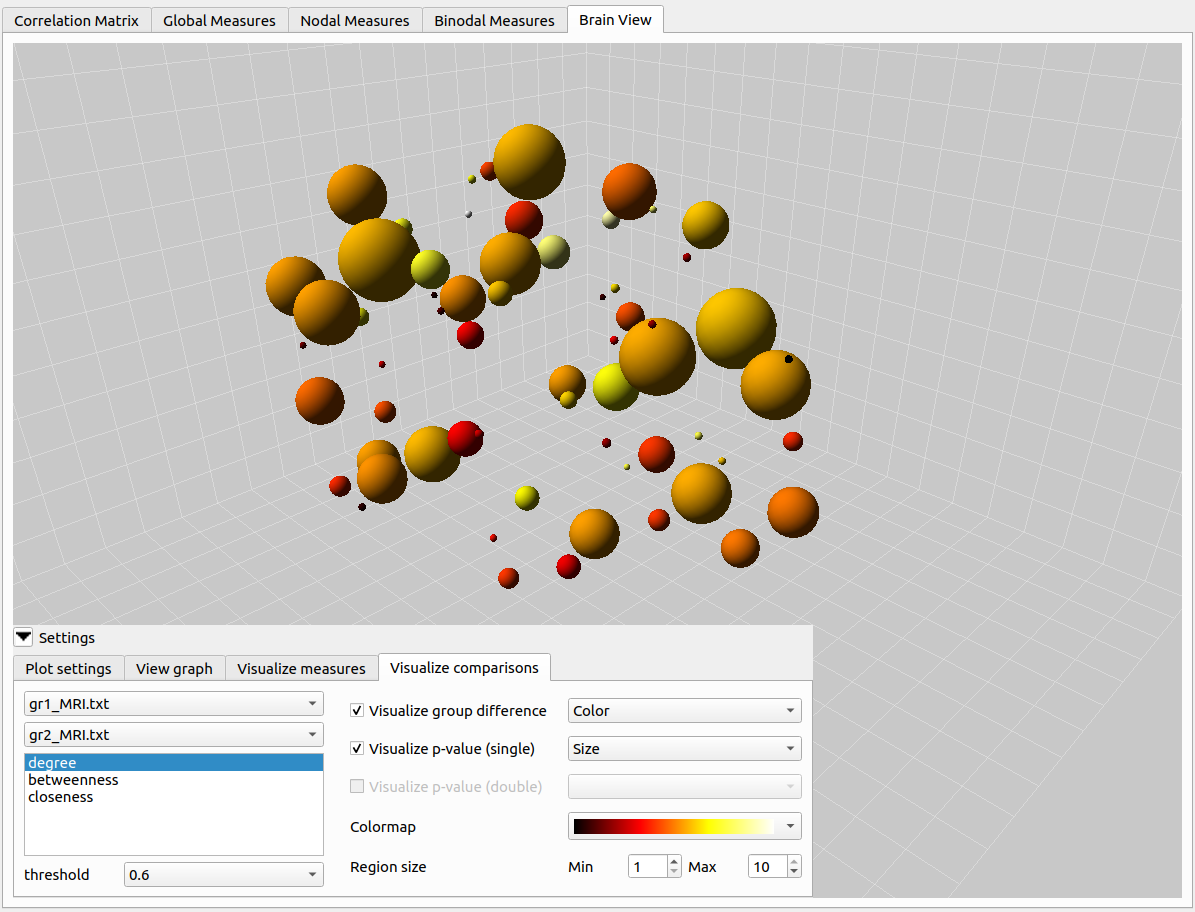
\includegraphics[width=0.7\linewidth]{comparison_vis.png}
    \caption{Visualization of nodal comparisons.}
    \label{fig:comparison_vis}
\end{figure}

\section{fMRI}

\subsection{fMRI Cohort}

The alterations in the fMRI Cohort Editor are very similar to the ones in the MRI Cohort Editor in Braphy. The GUI can be seen in \cref{fig:fmri_cohort}. One addition though is the 'Load subject group from folder' button. It lets the user select a whole folder of .xslx subject files and load them into the same group. As before, by pressing the 'Load subjects from file' button, the user can load .txt, .xml and .xlsx files. Here, one or several files can be selected. Each file will become a separate group. 

We do not have a window for the repetition time here yet, as we have not fully understood what meaning it has.

In the 'Subject data' tab, an additional button has been added to remove rows, see \cref{fig:fmri_cohort} at the bottom right.

\begin{figure}[H]
    \centering
    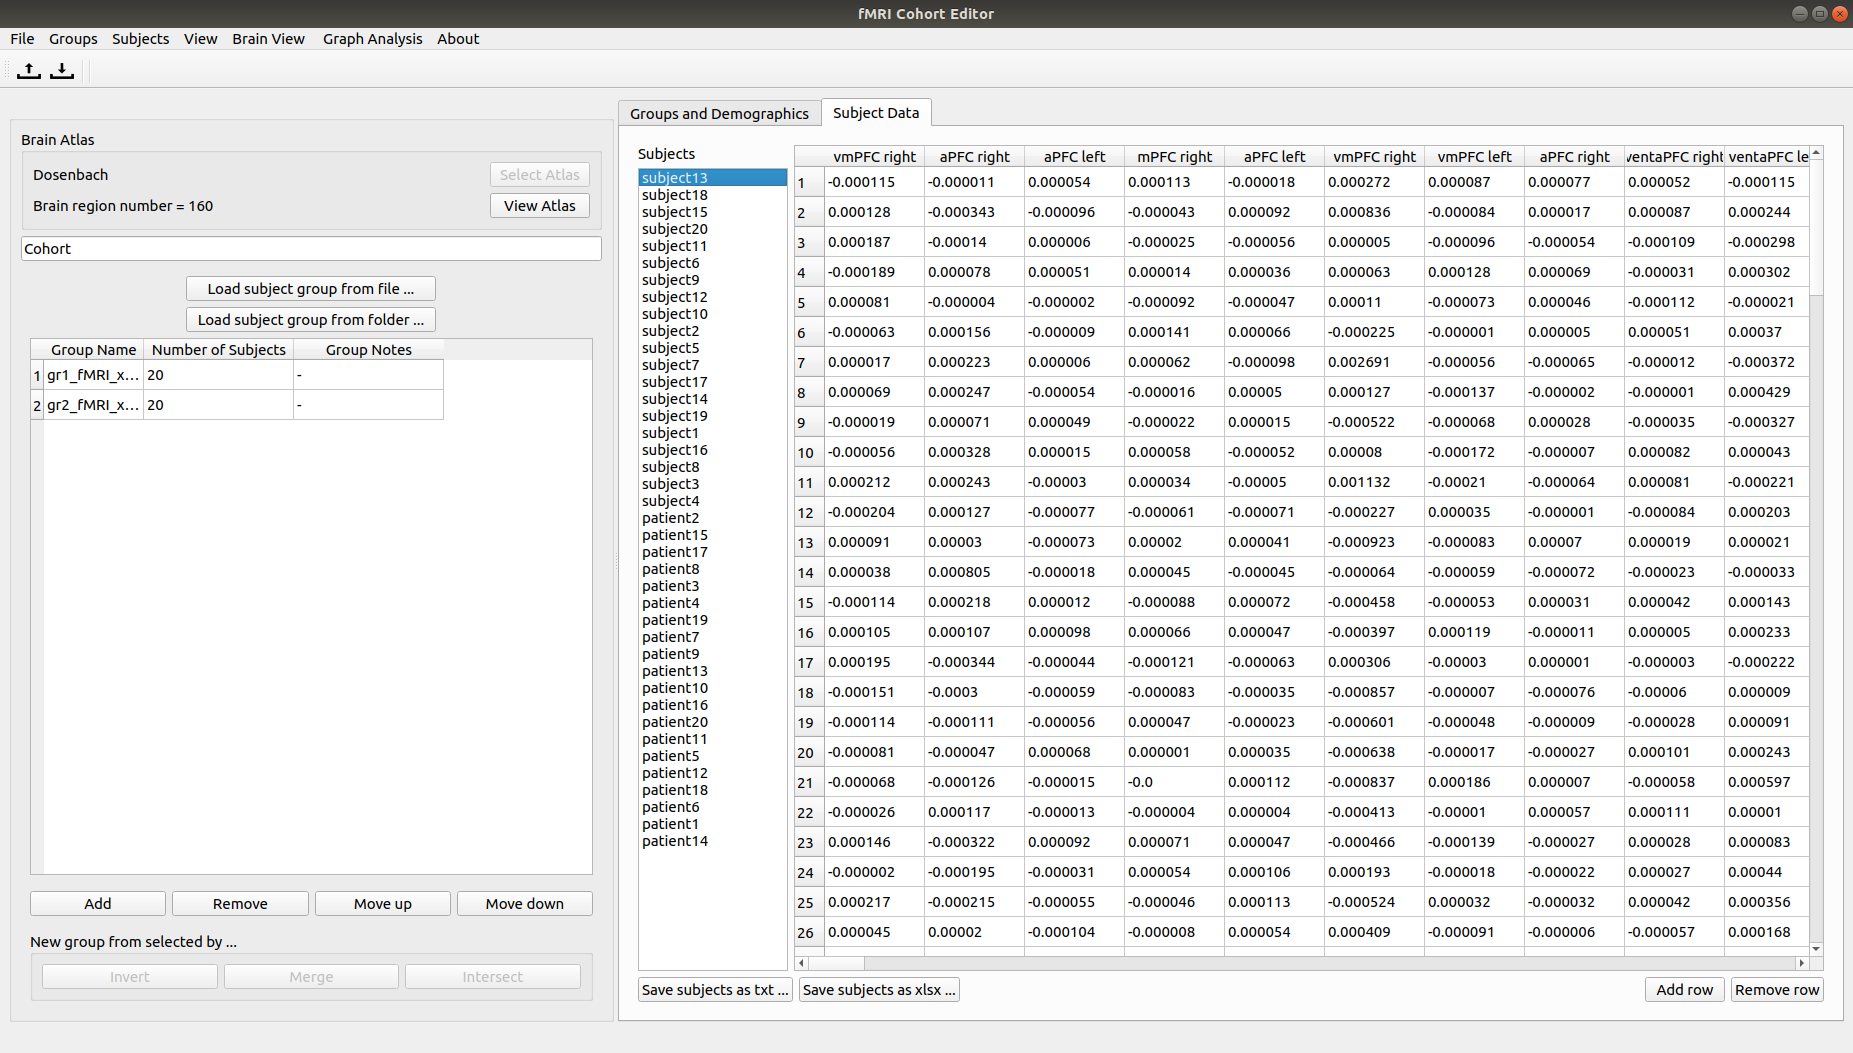
\includegraphics[width=\linewidth]{fmri_cohort.png}
    \caption{Visualization of nodal comparisons.}
    \label{fig:fmri_cohort}
\end{figure}

\subsection{fMRI Graph Analysis}

The Graph Analysis for fMRI in Braphy is basically equivalent to the one for MRI, described in \cref{sec:mri_ga}. This section will describe a few differences between them. 

First of all, there are no fMRI cohort files available in the repository. This is simply because they are too big to be added on GitHub. Instead, use the fMRI Cohort Editor to create a cohort.

Once the cohort is loaded, the fMRI Graph Analysis GUI looks like \cref{fig:fmri_ga}. To the right, in the visualization of the correlation matrix, the user can choose to visualize either the average correlation for the chosen group, or the correlation of a specific subject. We have chosen to add two radio buttons here to make it a bit more intuitive to choose settings.

\begin{figure}[H]
    \centering
    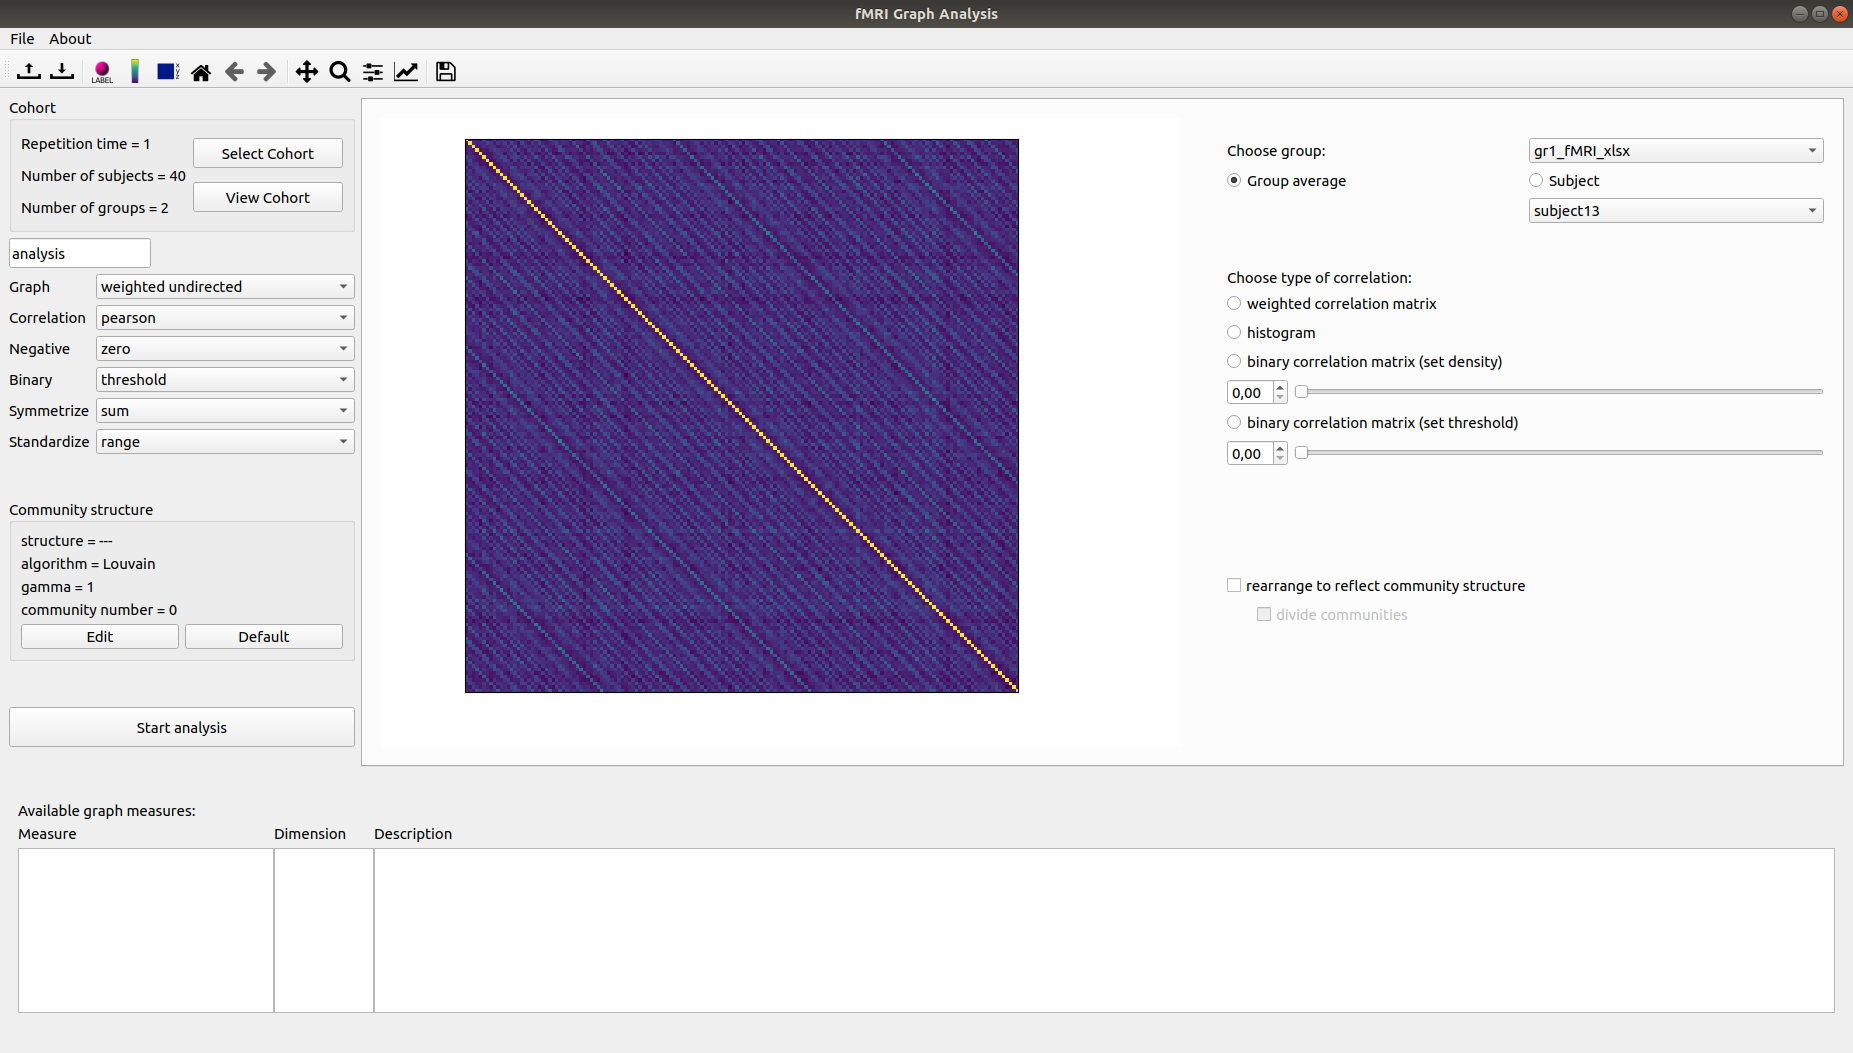
\includegraphics[width=0.9\linewidth]{fmri_ga.png}
    \caption{The fMRI Graph Analysis GUI after a cohort has been loaded.}
    \label{fig:fmri_ga}
\end{figure}


\subsubsection{Community Structure GUI}

In the community structure GUI for fMRI, see \cref{fig:fmri_cs}, the user can choose between computing and saving the communities for the whole group, using the average correlation matrix, or to set a separate community for each subject. If the 'Group average' radio button is checked, the button at the bottom left says "Set for current group". If the 'Subject' radio button is checked, the button says "Set for current subject" instead. 

\begin{figure}[H]
    \centering
    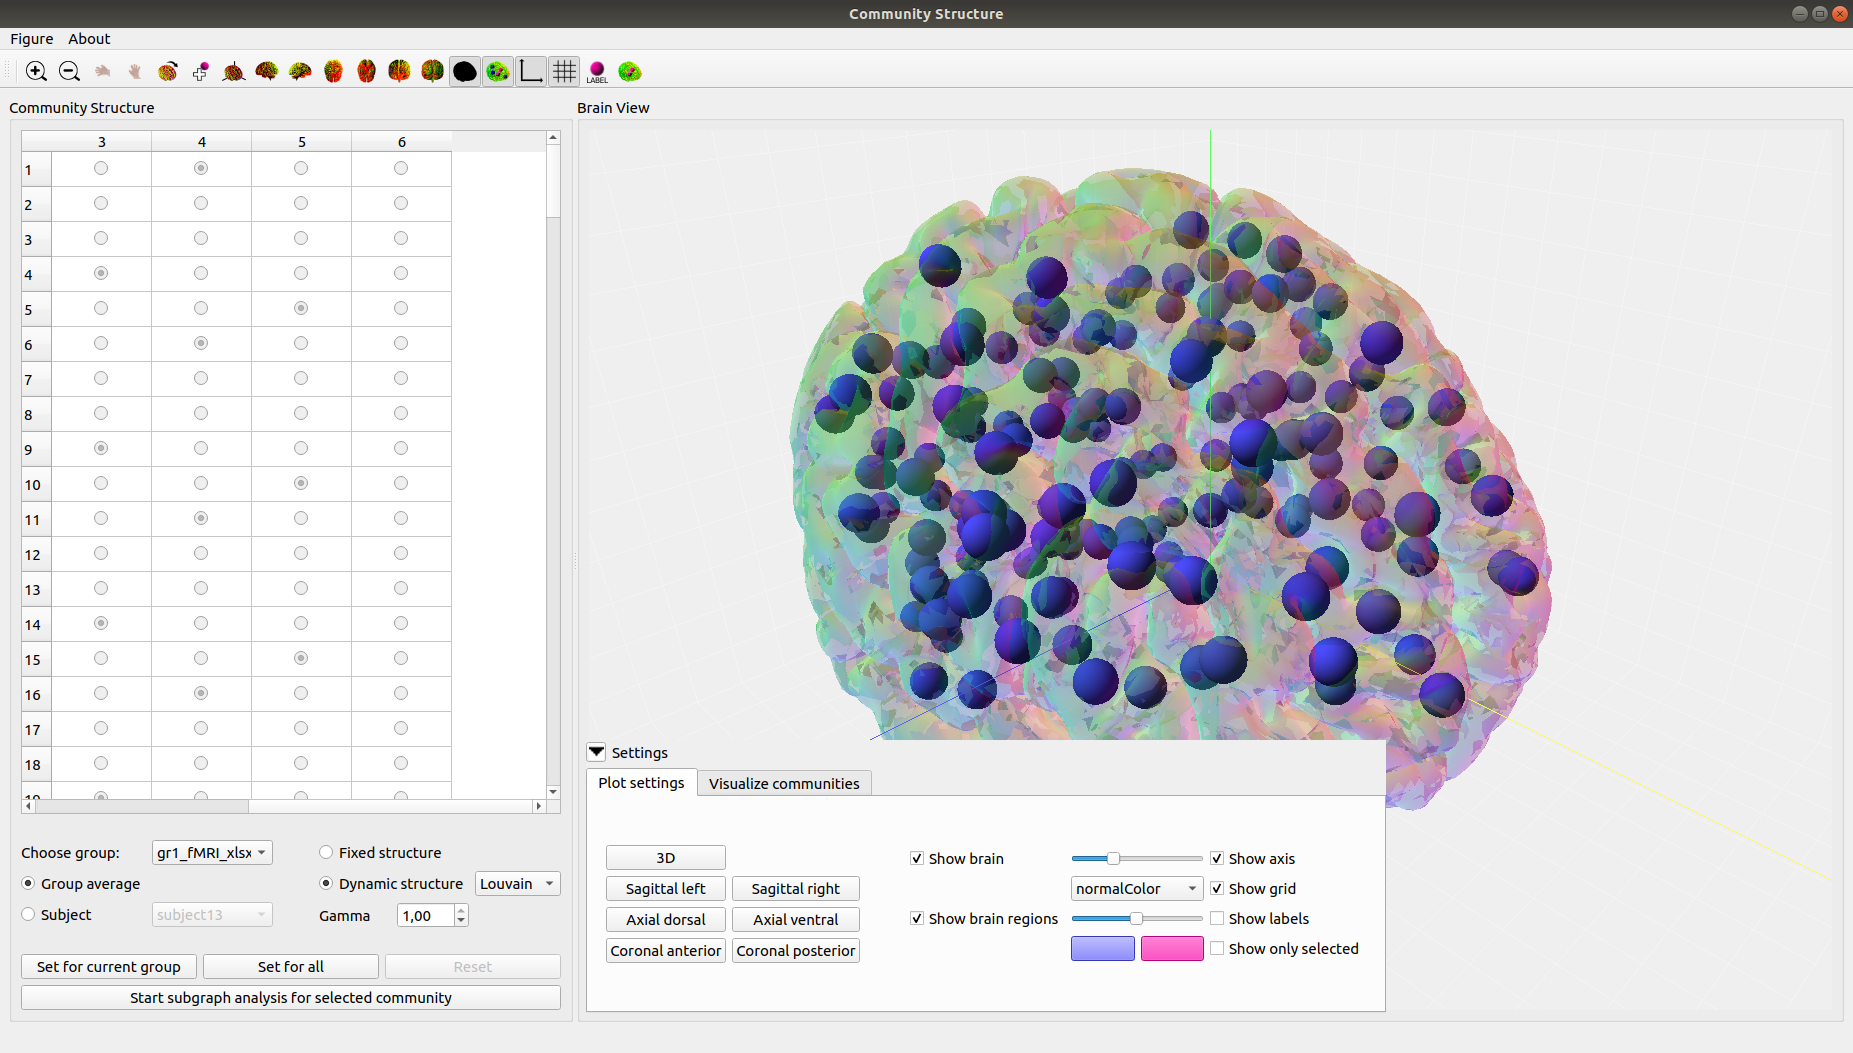
\includegraphics[width=0.9\linewidth]{fmri_cs.png}
    \caption{The fMRI Community Structure GUI. Note that the communities can be computed for the average correlation of a group or for each subject separately.}
    \label{fig:fmri_cs}
\end{figure}

\subsubsection{Start Analysis}

The computation of measures etc works almost the same as for MRI. In  the tables were the computed values are displayed, you can now choose to visualize either group averages or separate subjects, see \cref{fig:fmri_sa}. In the brain view tab, you can also visualize the graph of either the group average or separate subjects. Though, in the visualization of measures and comparisons in the brain view tab, only group averages can be visualized. If desired, the ability to choose a separate subject here could be added in the future.

\begin{figure}[H]
    \centering
    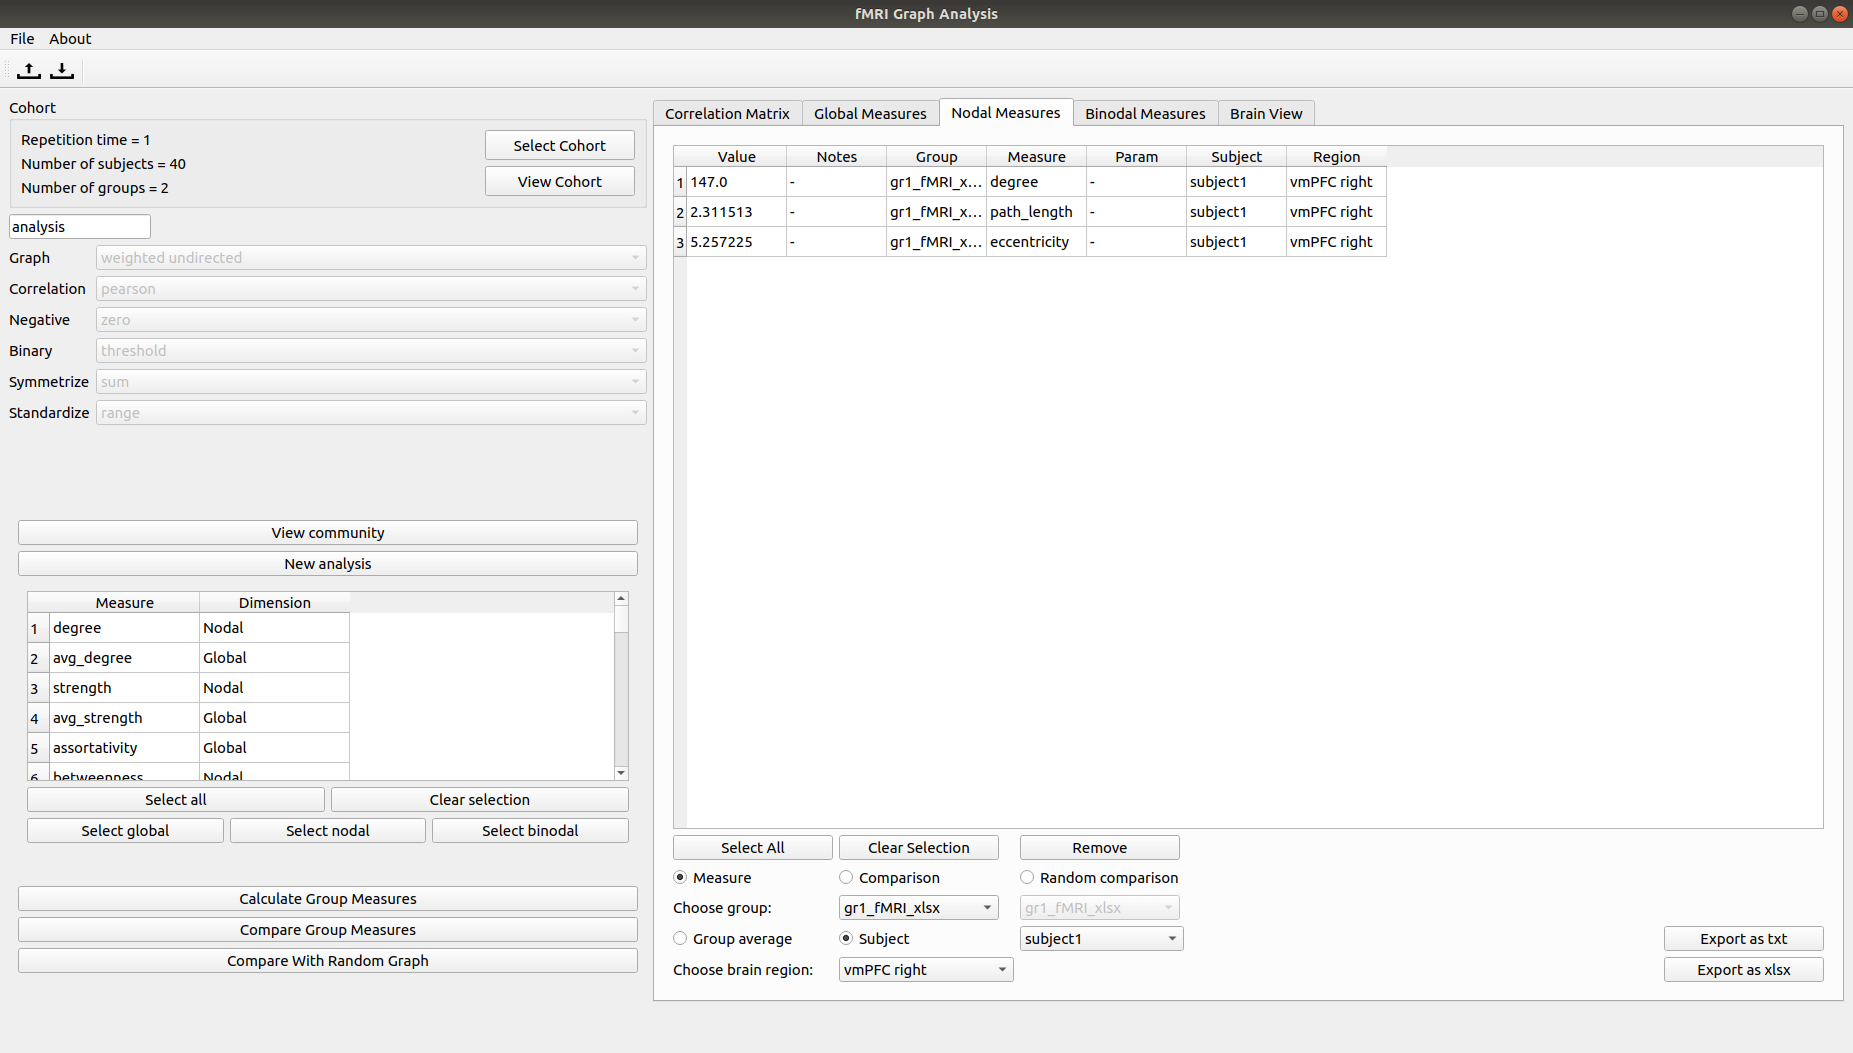
\includegraphics[width=\linewidth]{fmri_sa.png}
    \caption{The fMRI Graph Analysis GUI after the 'Start Analysis' button has been pressed. Note that the measures and comparisons can be displayed as group averages or for each subject separately.}
    \label{fig:fmri_sa}
\end{figure}

\end{document}
